\Needspace{8\baselineskip}
\subsection{问题二：跨维度数据融合与广义标度律}
\begingroup
\setlength{\tabcolsep}{2pt}
\clubpenalty=10000
\widowpenalty=10000

\subsubsection{具体分析}

即使模型大小和训练数据量相同，换用不同语料后，验证损失也可能变化。因此，本问在规模关系之外加入质量和领域配比，进一步比较改善数据与增加参数能否取得相近效果。附件 A 记录配比实验，附件 B 记录规模与质量实验，两者没有同时观测全部变量，连接时需要说明评分是否可比、配比效果能否迁移。

我们的处理顺序见图\ref{fig:p2_framework}。先检查各数据集的用途和质量方向，再利用 Pythia 轨迹拟合规模关系，并把较大模型留出检验。随后对比四种质量表达，选择广义标度律，利用弹性和等损失公式解释质量投入的效果。最后接入问题一的配比系数，并用不同来源的检验结果说明模型适合在哪些条件下使用。

\begin{figure}[!htbp]
  \centering
  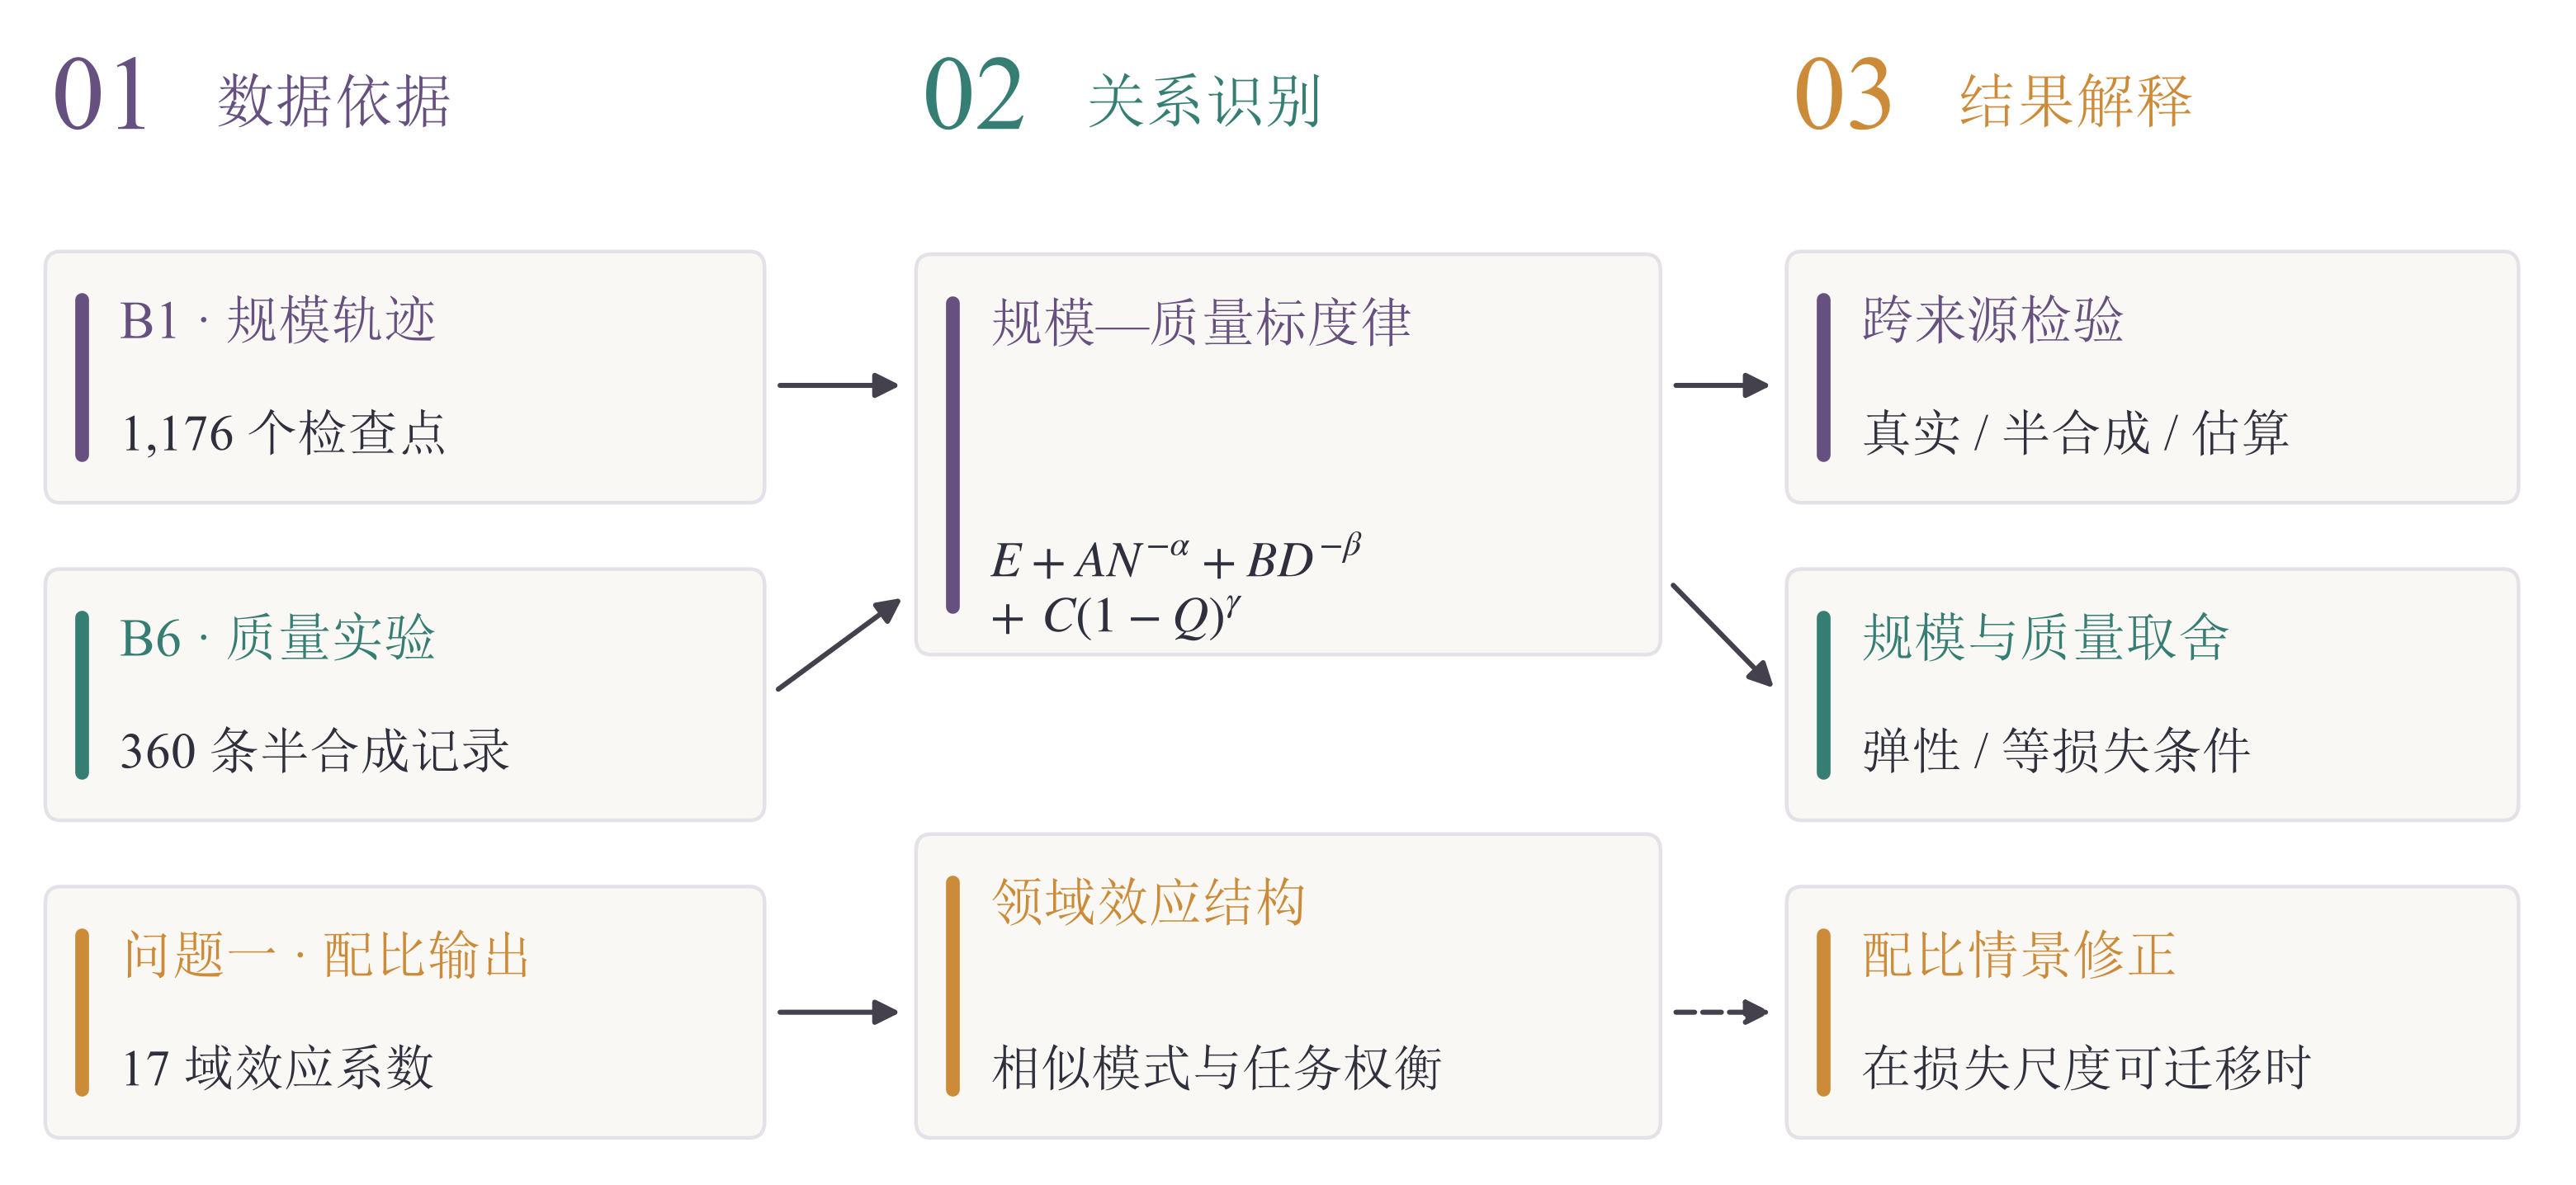
\includegraphics[width=0.98\textwidth]{../求解/问题二/图片/图0_问题二分析框架.png}
  \caption{规模、质量与领域效应的分析框架}
  \label{fig:p2_framework}
\end{figure}

\subsubsection{模型准备}

\textbf{1.数据组织与变量口径}\par\nopagebreak[4]
估计规模项采用 B1，其中包含 8 个 Pythia 模型，每个模型有 147 个检查点，共 1{,}176 条记录\cite{biderman2023pythia}。质量项采用 B6 半合成实验，B7 中与 B6 重复的记录不再用于扩展检验。其余附件分别承担对照作用：B2、B3 检查训练轨迹，B4、B5 检查跨族和文献数据，B8 检查质量评分是否同向；B9、B10 配对后用于比较大规模模型的估算损失。

我们用 $N$、$D$、$Q$ 分别表示参数量、训练数据量和质量，预测量为验证集交叉熵损失 $L$。本节的 $N$ 以十亿参数计，$D$ 以十亿 tokens 计；问题三计算算力时，两者均需乘以 $10^9$，恢复为绝对数量。拟合直接使用包含常数项 $E$ 的原函数，以保留不可约损失，避免取双对数时遗漏这一项。

\textbf{2.质量字段方向检验}\par\nopagebreak[4]
质量分数的含义需要先从数据中检查。固定每组实验的 $(N,D)$，计算组内 $Q_{\text{score}}$ 与损失的 Pearson 相关，再对各组系数取算术平均。平均相关为负，表示高评分通常对应低损失，符合本文的质量定义；若为正，则需要核对评分方向。表\ref{tab:p2_dir}中的均值只描述这一方向，不用于判断统计显著性。

\begin{table}[htbp]
  \centering
  \caption{质量评分方向与样本使用方式}
  \label{tab:p2_dir}
  \renewcommand{\arraystretch}{1.15}
  \setlength{\tabcolsep}{5pt}
  \begin{tabularx}{0.98\textwidth}{@{}
    >{\hsize=0.65\hsize\linewidth=\hsize\centering\arraybackslash}X
    >{\hsize=0.65\hsize\linewidth=\hsize\centering\arraybackslash}X
    >{\hsize=0.70\hsize\linewidth=\hsize\centering\arraybackslash}X
    >{\hsize=2.00\hsize\linewidth=\hsize\raggedright\arraybackslash}X@{}}
    \toprule
    数据分组 & \makecell{平均组内\\相关系数} & \makecell{记录数 /\\实验组数} & 评分解释与使用方式 \\
    \midrule
    B6 & $-0.925$ & 360 / 45 & 沿用原评分；$Q=1$ 为最优参考 \\
    B7 & $-0.918$ & 450 / 45 & 与 B6 同向，仅新增记录用于检验 \\
    B8 校准段 & $+0.995$ & 984 / 90 & 方向相反，翻转评分后作诊断 \\
    B8 外推段 & $+0.968$ & 720 / 60 & 方向相反，不纳入主拟合 \\
    \bottomrule
  \end{tabularx}
  \par\smallskip
  \begin{minipage}{0.98\textwidth}\normalsize
  注：实验组固定 $N,D$。B7 包含 B6 的全部 360 条记录，新增 90 条；均值只描述方向，不表示显著性。
  \end{minipage}
\end{table}

表中 B6 和 B7 分别得到 $-0.925$、$-0.918$，因此使用原评分 $Q=Q_{\text{score}}$。逐行比对发现，B7 已含 B6 的全部 360 条记录，只有另外 90 条可用于扩展检查，两套数据不能算作独立证据。B8 的两个子集方向相反，部分损失还低于本模型的下限。我们不把 B8 加入主拟合，只将评分改为 $1-Q_{\text{score}}$，检查翻转后是否仍存在偏差。

图\ref{fig:p2_direction}中，每个圆点对应一组固定 $(N,D)$ 的实验，菱形表示各组相关系数的平均值。B6/B7 的点大多在零点一侧，B8 则在另一侧，说明方向差异并非由少数组造成。B6 与 B7 的点群相近还与记录重叠有关，不能把这种接近当成新增的独立验证。

\begin{figure}[!htbp]
  \centering
  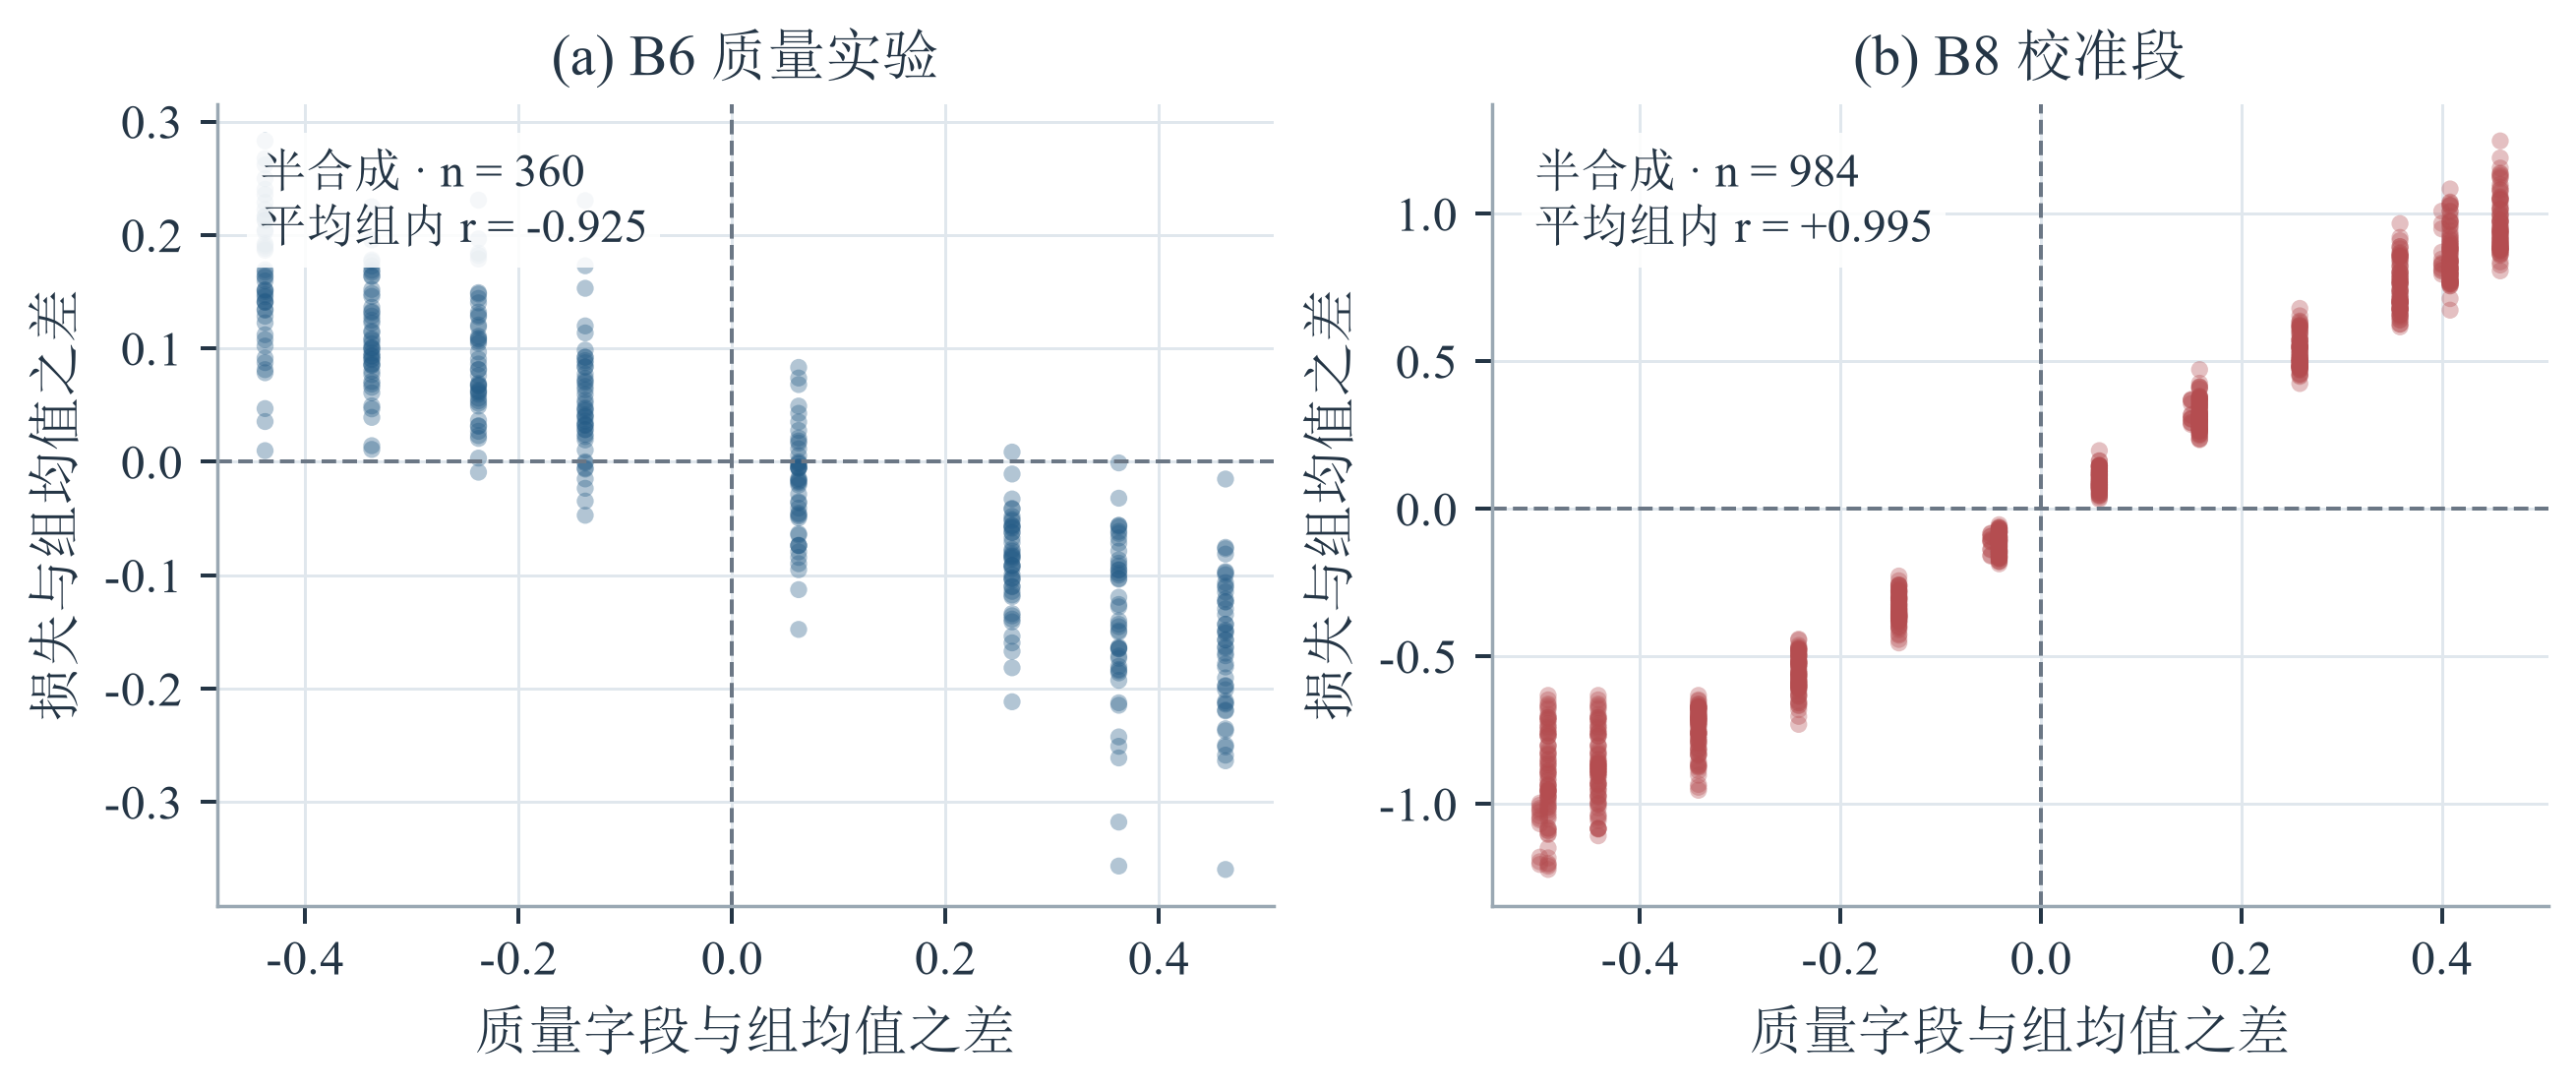
\includegraphics[width=0.98\textwidth]{../求解/问题二/图片/图7_质量方向对照.png}
  \caption{质量字段与损失的组内相关分布}
  \label{fig:p2_direction}
\end{figure}

\begin{samepage}
统一方向只解决了分数高低的含义，还不能保证不同评分可以直接互换。问题一的综合评分与附件 B 的 $Q_{\text{score}}$ 来自不同构造方法，相同分值未必对应相同质量。因此，本节的质量参数和数值解释均使用附件 B 的评分尺度。
\par
\end{samepage}

\subsubsection{模型建立}

\textbf{1.经典标度律}\par\nopagebreak[4]
先在参考质量下考察规模效应。采用 Chinchilla 标度律\cite{hoffmann2022chinchilla}，把验证损失 $L$ 写成参数量与数据量的函数：
\begin{equation}
    L(N,D) = E + \frac{A}{N^{\alpha}} + \frac{B}{D^{\beta}}
\end{equation}
式中，$E$ 是 $N,D\to\infty$ 时仍保留的损失。其余两项分别随参数量和数据量增加而下降，变化速度由 $\alpha$、$\beta$ 控制，幅度由 $A$、$B$ 控制。固定参考质量后，便可以分别比较增加参数和增加数据的收益。

\textbf{2.质量项的选择与损失修正}\par\nopagebreak[4]
加入质量有两种常见思路：让质量改变有效规模，或用单独一项表示质量不足的损失。本文在同一组联合样本上比较四种形式，依据 B6 的拟合、B7 新增点的预测相关和残差信息评分作选择，结果见表\ref{tab:p2_form}。各候选模型和经典模型均用带界约束的非线性最小二乘估计，保留常数与幂函数项，并采用 soft-$L_1$ 损失减轻大残差的影响。

\begin{table}[htbp]
  \centering
  \caption{不同质量作用形式的拟合与扩展检验指标}
  \label{tab:p2_form}
  \renewcommand{\arraystretch}{1.15}
  \begin{tabularx}{0.98\textwidth}{@{}>{\raggedright\arraybackslash}X*{4}{>{\centering\arraybackslash}p{0.17\textwidth}}@{}}
    \toprule
    比较指标 & \makecell{加性质量缺口\\$C(1-Q)^\gamma$} & \makecell{质量同时乘\\$N$ 与 $D$} & \makecell{加性质量亏损\\$CQ^{-\gamma}$} & \makecell{质量作为\\有效数据乘子} \\
    \midrule
    联合样本 $R^2$ & \textbf{0.9896} & 0.9882 & 0.9848 & 0.9745 \\
    B6 样本 $R^2$ & \textbf{0.9556} & 0.9495 & 0.9349 & 0.8905 \\
    B7 新增点 $r$ & 0.991 & \textbf{0.991} & 0.991 & 0.983 \\
    待估参数个数 & 7 & 7 & 7 & 6 \\
    残差信息评分 $I_{\mathrm{RSS}}$ & $\mathbf{-10236}$ & $-10042$ & $-9660$ & $-8866$ \\
    \bottomrule
  \end{tabularx}
  \par\smallskip
  \begin{minipage}{0.98\textwidth}\normalsize
  注：相关系数保留三位小数；加粗的最优指标按未舍入值确定。$I_{\mathrm{RSS}}$ 越小越优，仅用于同样本比较。
  \end{minipage}
\end{table}

\begin{samepage}
四种形式在 B7 新增点上的相关系数都不低于 $0.983$，这一指标不足以单独决定选择。表\ref{tab:p2_form}中，加性质量缺口形式在联合样本和 B6 上的 $R^2$ 均最高，因此采用该形式。后续同时报告 RMSE 和 MAPE，检查较高相关是否伴随较小的实际预测误差。
\par
\end{samepage}

\begin{samepage}
残差信息评分采用 $I_{\mathrm{RSS}}=n\ln(\mathrm{RSS}/n)+2k$，其中 $n$ 为样本数，$k$ 为参数数。参数通过 soft-$L_1$ 而非高斯极大似然估计，所以该值只用于相同样本下的辅助比较，不按严格的 AIC 解释。另外，B7 新增记录既参与形式选择，也参与扩展检查，其结果属于开发阶段验证，不能作为完全独立的最终测试。
\par
\end{samepage}

将选定的质量缺口项加入规模基线后，损失关系写为：
\begin{equation}
    L(N,D,Q) = E + \frac{A}{N^{\alpha}} + \frac{B}{D^{\beta}} + C\,(1-Q)^{\gamma},
    \qquad C>0,\ \gamma>0
\end{equation}
\begin{samepage}
将 $Q=1$ 设为质量参考点，使质量项在此处归零，广义模型便恢复经典标度律的形式。联合拟合会重新估计参数，不要求与经典拟合值相同。Pythia 没有质量实测值，赋予 $Q=1$ 也仅表示这一参考约定。固定 $Q$，令参数和数据量同时增大，可得
\par\nopagebreak[4]
\begin{equation}
    \lim_{N,D\to\infty} L(N,D,Q) = E + C\,(1-Q)^{\gamma} \;\ge\; E
\end{equation}
\end{samepage}
由此可见，只要质量固定在 $Q<1$，扩大模型和增加数据都只能降低各自的规模项，质量缺口仍然存在。因此，在本加性模型中，规模投入不能完全消除质量不足的影响。该判断是函数结构的结果，应用到实际训练仍需考虑拟合范围。

\textbf{3.边际效用与弹性}\par\nopagebreak[4]
为刻画各因素微小变化对损失的影响，对广义模型求偏导，并在参考点 $(N_0,D_0,Q_0)$ 处评价：
\begin{equation}
    \frac{\partial L}{\partial N} = -\alpha A N^{-\alpha-1},\quad
    \frac{\partial L}{\partial D} = -\beta B D^{-\beta-1},\quad
    \frac{\partial L}{\partial Q} = -\gamma C (1-Q)^{\gamma-1}
\end{equation}
各偏导的单位不同。令参考点的预测损失为 $L_0$，按变量与损失的比例变化定义弹性：
\begin{equation}
    \varepsilon_N = \frac{\partial L}{\partial N}\frac{N_0}{L_0},\qquad
    \varepsilon_D = \frac{\partial L}{\partial D}\frac{D_0}{L_0},\qquad
    \varepsilon_Q = \frac{\partial L}{\partial Q}\frac{Q_0}{L_0}
\end{equation}

\textbf{4.质量提升与参数扩张的等效条件}\par\nopagebreak[4]
为了比较两种投入，固定 $D$ 与领域配比，并选择相同的初始配置。若少量提高质量和少量增加参数带来的损失降幅相等，就可用正向增量比 $R_{NQ}$ 表示其等效关系：
\begin{equation}
    \begin{aligned}
      \left|\frac{\partial L}{\partial Q}\right|\mathrm dQ
      &=\left|\frac{\partial L}{\partial N}\right|\mathrm dN_{\mathrm{eq}},\\
      R_{NQ}=\frac{\mathrm dN_{\mathrm{eq}}}{\mathrm dQ}
      &=\frac{\gamma C(1-Q)^{\gamma-1}}{\alpha A N^{-\alpha-1}}
       =\frac{\gamma C}{\alpha A}(1-Q)^{\gamma-1}N^{\alpha+1}.
    \end{aligned}
\end{equation}
$R_{NQ}$ 比较的是两种改善方案各自需要的增量。若要求损失保持不变，则应写为 $\mathrm dN/\mathrm dQ=-R_{NQ}$，即提高质量后可以减少参数。固定 $Q$ 时，该比值随 $N^{\alpha+1}$ 增长，因为大模型继续扩容的边际收益较小。这里的“等效”只针对损失，实际算力是否相等还要比较语料处理和训练成本。

当质量变化 $\Delta Q$ 不够小时，需要直接计算完整损失差。记质量改善带来的降幅为 $\delta_Q$，令参数扩张取得相同降幅，解得
\begin{equation}
  \begin{aligned}
    \delta_Q &= C\bigl[(1-Q)^\gamma-(1-Q-\Delta Q)^\gamma\bigr],\\
    \Delta N_{\mathrm{eq}}
      &= N\left[\left(1-\frac{\delta_Q N^\alpha}{A}\right)^{-1/\alpha}-1\right].
  \end{aligned}
  \label{eq:p2_finite}
\end{equation}
首先要求 $0<\Delta Q\leq1-Q$，以免质量超过上界。其次，只有 $\delta_Q<AN^{-\alpha}$ 时，才能找到有限的等效参数增量；两者相等时需要无限参数，前者更大时则没有仅靠扩容的等效解。原因是当前参数项 $AN^{-\alpha}$ 已是扩容所能消除的全部损失。当 $\Delta Q\to0$，上式回到局部近似 $\Delta N_{\mathrm{eq}}\approx R_{NQ}\Delta Q$；计算结果若超过拟合规模，仍需按外推看待。


\textbf{5.领域效应的相似性}\par\nopagebreak[4]
同一训练领域在不同验证任务上的作用也可能不同。问题一给出了领域 $i$、$j$ 在 13 个任务上的系数向量 $\bm a_i,\bm a_j$。先减去平均向量，再用余弦相似度比较它们的相对作用：
\begin{equation}
    s_{ij} = \frac{\langle \bm a_i-\bar{\bm a},\ \bm a_j-\bar{\bm a}\rangle}{\|\bm a_i-\bar{\bm a}\|\,\|\bm a_j-\bar{\bm a}\|}
\end{equation}
$\bar{\bm a}$ 为 17 个训练领域系数向量的均值。$s_{ij}\to1$ 表示两域的相对作用方向接近，$s_{ij}\to-1$ 表示方向相反，可能涉及不同任务之间的取舍。余弦值没有保留作用大小，原回归也没有领域交互项。因此，仅凭相似度还不能确定两域可以等量替换，或联合使用后会获得额外收益。

\subsubsection{模型求解}

\noindent\textbf{辅助分析说明：} 本问数据整理、绘图与数值核对使用 Codex 辅助，模型为 GPT-5.4（OpenAI，2026-03-05）及 GPT-6 系列（OpenAI，2026-09-03 系列首次发布）\cite{ai_codex54,ai_codex6}。

\begin{samepage}
\textbf{1.经典标度律拟合与留出验证}\par\nopagebreak[4]
首先用 B1 的 1{,}176 条记录估计经典模型。图\ref{fig:p2_classic}左侧展示损失与两类规模的关系，右侧比较不同规模模型的残差，拟合得到
\begin{equation}
    L(N,D) = 1.6898 + \frac{0.3540}{N^{0.3400}} + \frac{1.2403}{D^{0.2799}}
\end{equation}
全部记录的拟合结果为 $R^2 = 0.9999998$、RMSE $=1.5\times10^{-4}$、MAPE $=0.004\%$。随后只用最小的 4 个模型重新估计，并预测留出的 4 个较大模型，得到 $R^2=0.9999997$、MAPE $=0.005\%$。误差仍较小，说明这一规模关系在所考察的 Pythia 模型族内保持稳定。
\par
\end{samepage}

\begin{figure}[!htbp]
  \centering
  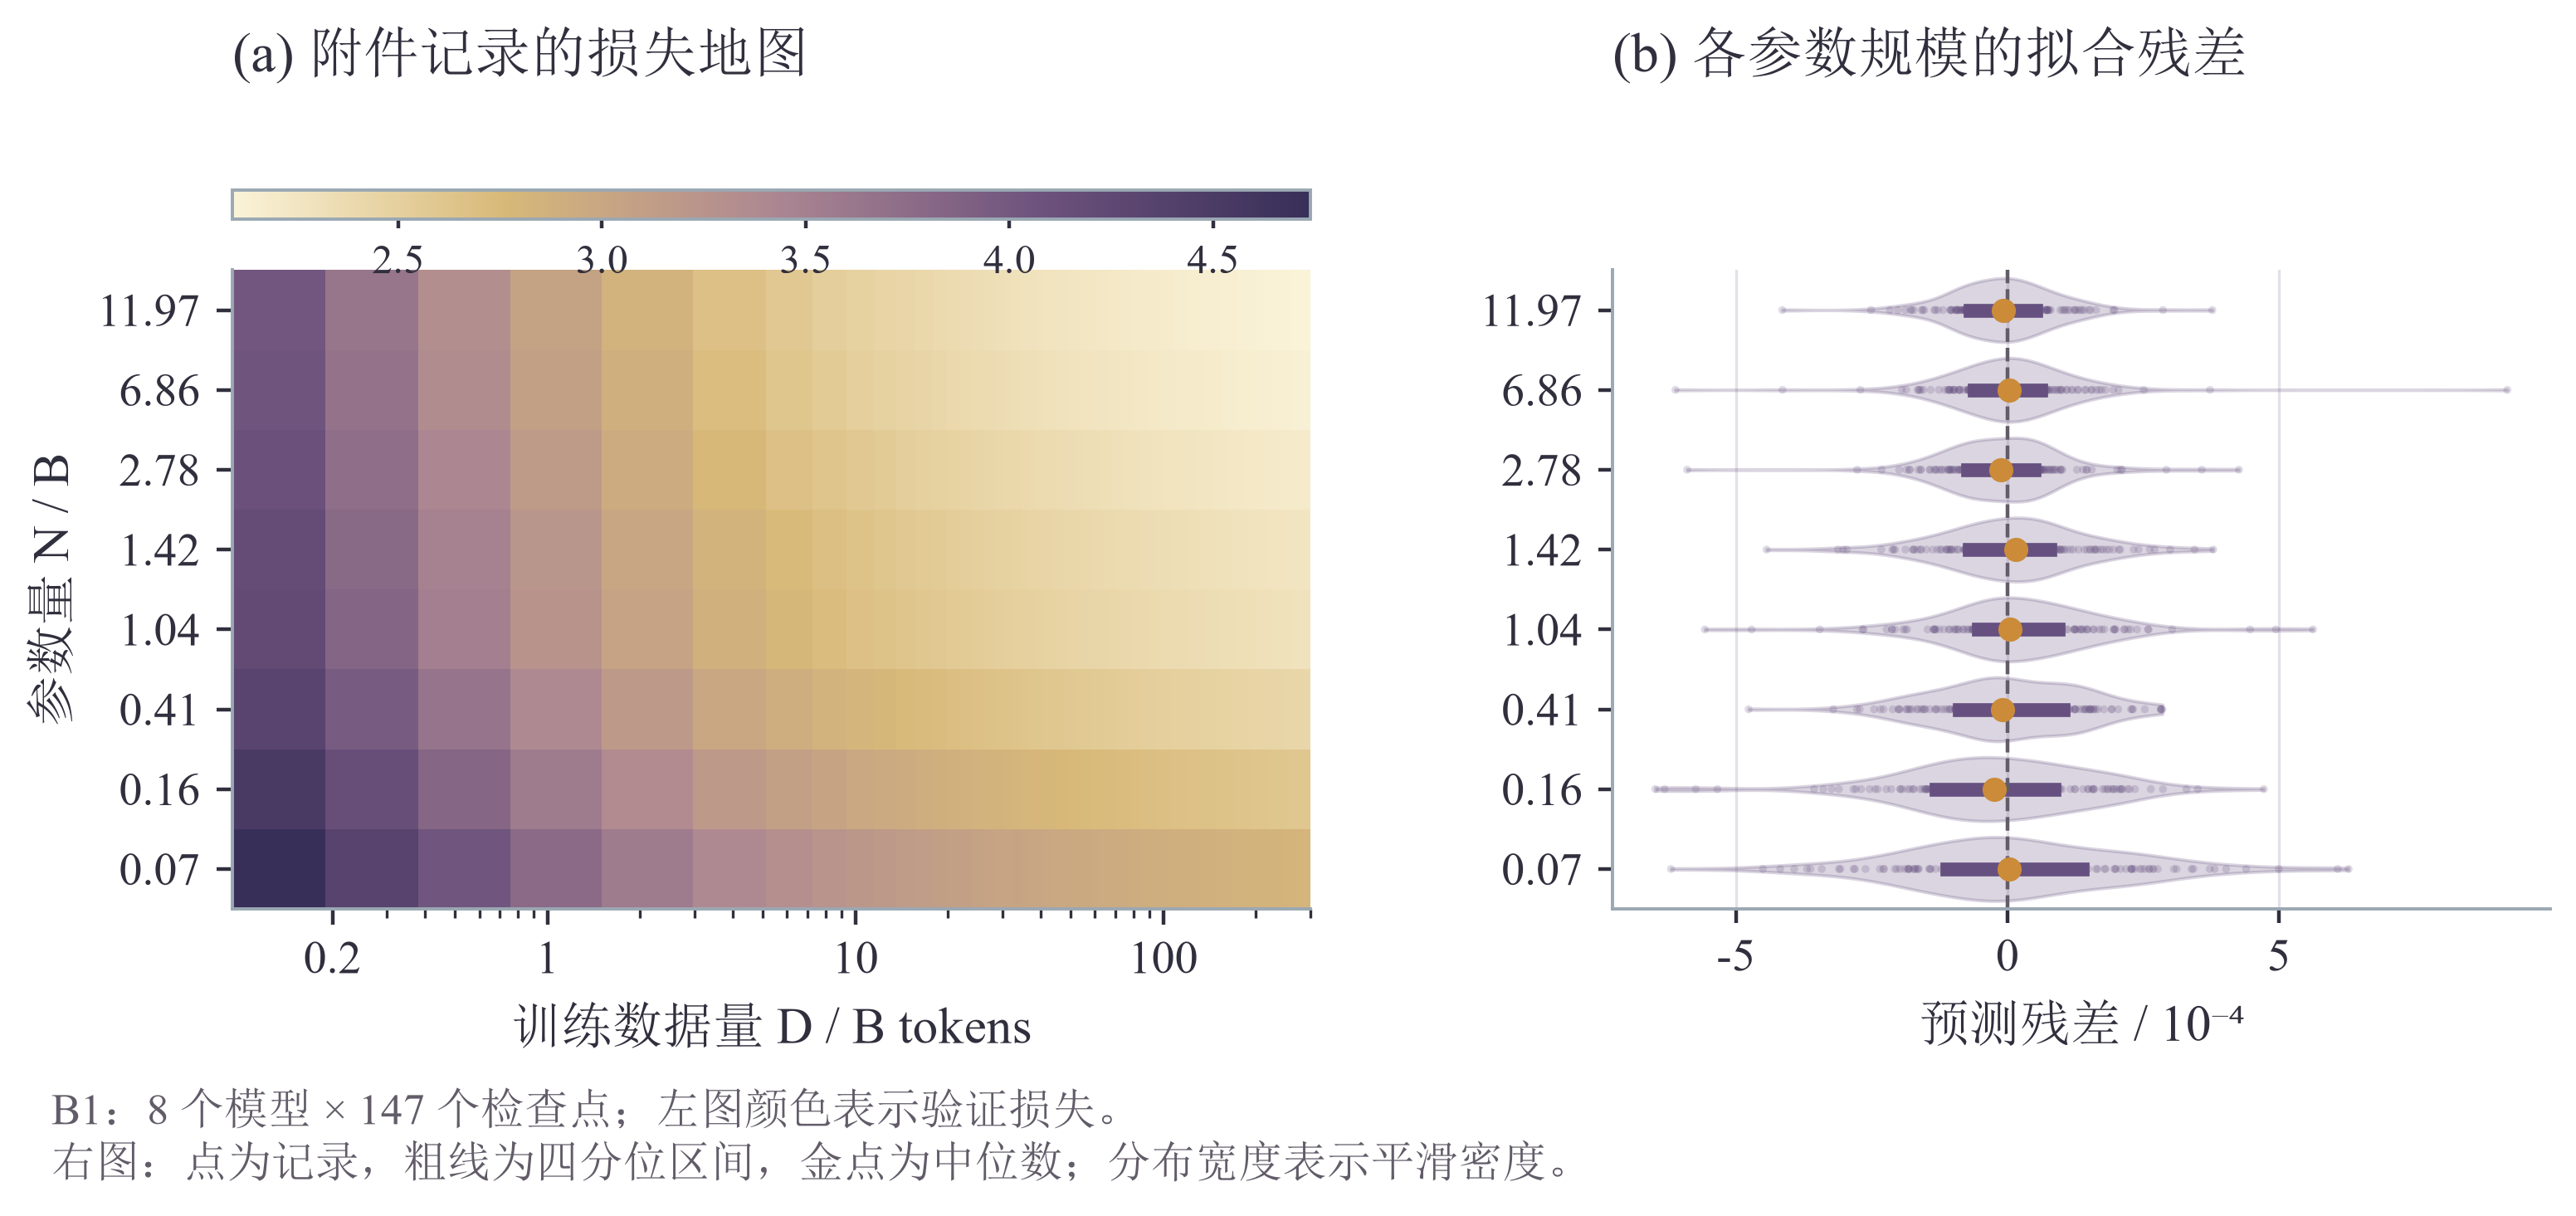
\includegraphics[width=0.98\textwidth]{../求解/问题二/图片/图1_经典标度律拟合.png}
  \caption{Pythia 规模--损失地图与分模型残差分布}
  \label{fig:p2_classic}
\end{figure}

残差标准差只有 $1.5\times10^{-4}$，远小于损失本身的标准差 $0.342$，所选函数与 B1 记录非常接近。但这还不能说明换用数据来源后仍有同等精度，故继续使用 B4、B5 外部数据和 B2 半合成轨迹检查。

\begin{samepage}
B3 可用于检查数据项的指数是否一致。分别固定 8 条插值轨迹的 $N$，先从损失中扣除 $E+AN^{-\alpha}$，再对 $L-(E+AN^{-\alpha})$ 与 $D$ 作双对数回归。所得指数为 $-0.2806\sim-0.2803$，与 $-\beta=-0.2799$ 接近。由于这些轨迹由 Pythia 检查点插值得到，结果说明内部关系一致，并不增加独立观测。
\par
\end{samepage}

\textbf{2.广义标度律参数估计}\par\nopagebreak[4]
再将 Pythia 的规模记录与 B6 质量实验合并，估计表\ref{tab:p2_form}选出的广义形式。对没有质量实测值的 Pythia 仍按约定取 $Q=1$，各项系数和指数列于表\ref{tab:p2_params}。

\begin{table}[H]
  \centering
  \caption{广义模型各损失项的参数配置}
  \label{tab:p2_params}
  \renewcommand{\arraystretch}{1.15}
  \setlength{\tabcolsep}{5pt}
  \begin{tabularx}{0.94\textwidth}{@{}*{5}{>{\centering\arraybackslash}X}@{}}
    \toprule
    损失组成 & 系数符号 & 系数估计 & 指数符号 & 指数估计 \\
    \midrule
    不可约损失 & $E$ & 1.6558 & -- & -- \\
    参数规模项 & $A$ & 0.3808 & $\alpha$ & 0.3266 \\
    训练数据项 & $B$ & 1.2515 & $\beta$ & 0.2767 \\
    质量缺口项 & $C$ & 0.3544 & $\gamma$ & 0.9779 \\
    \bottomrule
  \end{tabularx}
  \par\smallskip
  \begin{minipage}{0.94\textwidth}\normalsize
  注：联合拟合 $R^2=0.9896$；不可约损失为常数项，不含衰减指数。
  \end{minipage}
\end{table}

\begin{samepage}
联合估计得到 $R^2=0.9896$、RMSE $=0.036$ 和 MAPE $=0.66\%$。表\ref{tab:p2_params}中的 $\gamma=0.9779\approx1$，表示质量缺口扩大时，渐近损失近似按线性关系增加。这里增加了质量实验，样本已不同于经典拟合，所以不能用两个 $R^2$ 的差值衡量加入质量项的收益。
\par
\end{samepage}

\begin{samepage}
图\ref{fig:p2_quality}说明质量对损失的影响。左图固定 $D=300$B tokens，用底色和等值线表示不同规模、质量组合的预测损失，空心点为 B6 实验位置；右图以 $E$ 为起点，展示质量不足使损失下限增加多少。
\par
\end{samepage}

根据 $E+C(1-Q)^{\gamma}$，$Q=1$ 时损失下限为 $1.656$。质量分别降到 $Q=0.6$、$Q=0.3$ 后，下限提高至 $1.801$、$1.906$。

\begin{figure}[!htbp]
  \centering
  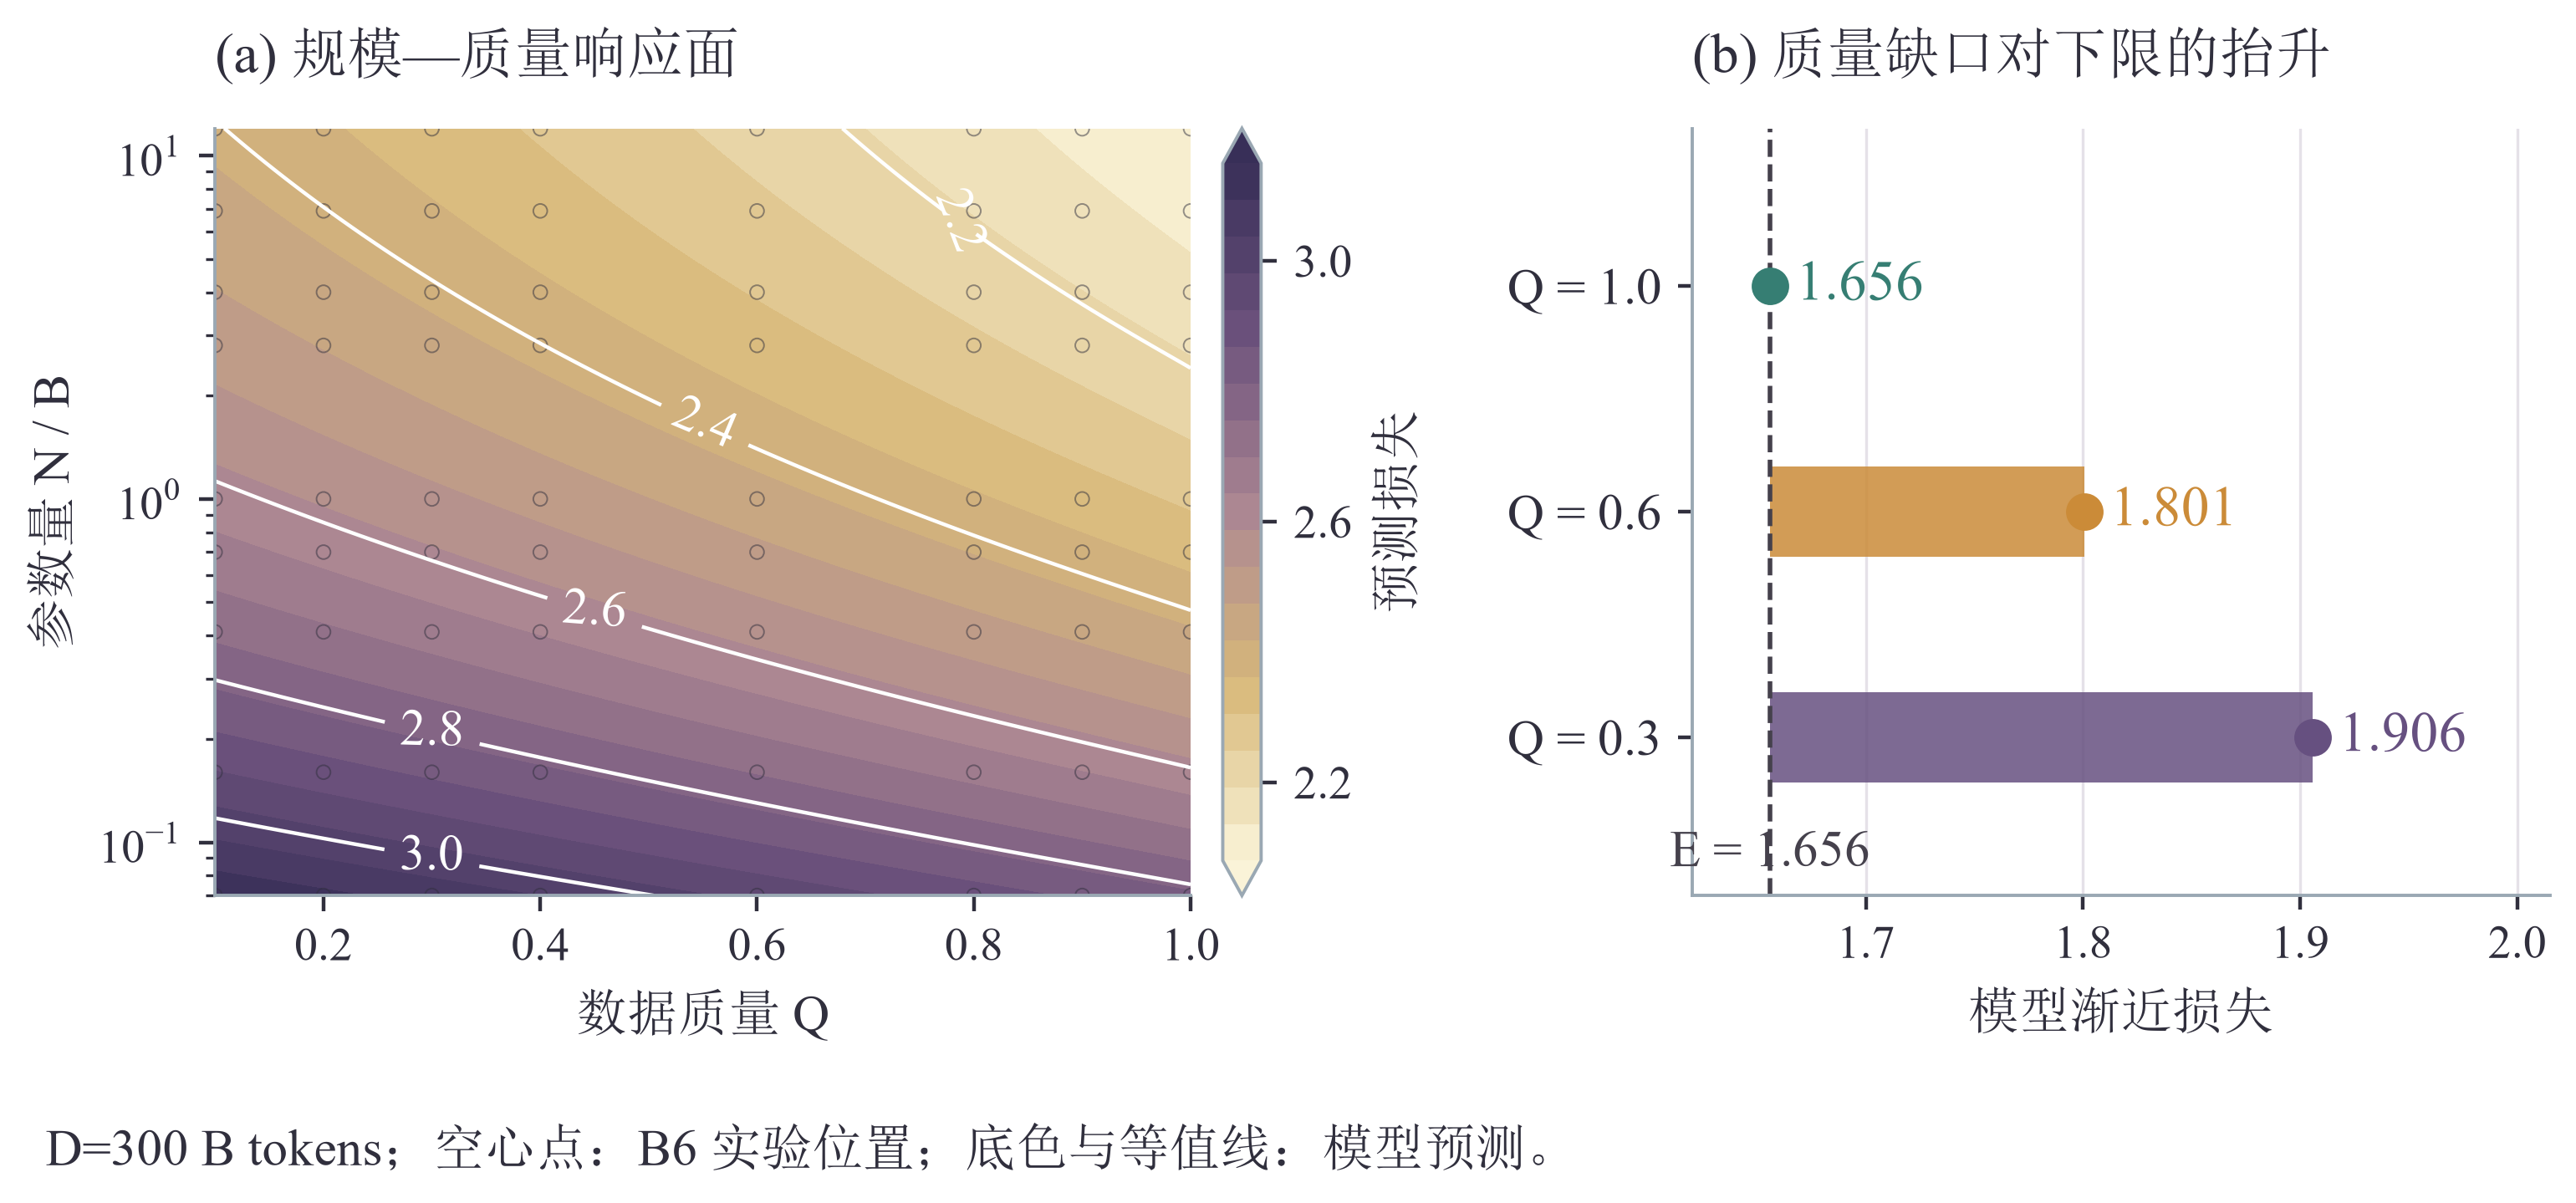
\includegraphics[width=0.98\textwidth]{../求解/问题二/图片/图3_质量边际影响.png}
  \caption{规模--质量响应面与渐近损失分解}
  \label{fig:p2_quality}
\end{figure}

\textbf{3.分层检验与适用范围}\par\nopagebreak[4]
配置计算依赖模型预测，因此还需比较不同来源上的误差。表\ref{tab:p2_val}汇总 6 组检验的 MAPE、RMSE 和相关系数，图\ref{fig:p2_general}展示 $100(\hat L-L)/L$ 的分布：负值为低估，正值为高估。为同时看清小误差和大偏差，图中横轴在 $\pm10\%$ 内采用线性刻度，外侧改用对称对数刻度。

\begin{table}[htbp]
  \centering
  \caption{按数据性质区分的预测误差与相关性}
  \label{tab:p2_val}
  \renewcommand{\arraystretch}{1.15}
  \setlength{\tabcolsep}{5pt}
  \begin{tabularx}{0.98\textwidth}{@{}
    >{\hsize=0.75\hsize\linewidth=\hsize\centering\arraybackslash}X
    >{\hsize=2.25\hsize\linewidth=\hsize\raggedright\arraybackslash}X
    >{\hsize=0.75\hsize\linewidth=\hsize\centering\arraybackslash}X
    >{\hsize=0.80\hsize\linewidth=\hsize\centering\arraybackslash}X
    >{\hsize=0.75\hsize\linewidth=\hsize\centering\arraybackslash}X
    >{\hsize=0.70\hsize\linewidth=\hsize\centering\arraybackslash}X@{}}
    \toprule
    数据性质 & 对照样本 & 记录数 & MAPE/\% & RMSE & $r$ \\
    \midrule
    \multirow{2}{*}{真实} & B4 跨模型族收敛点 & 57 & 8.8 & 0.293 & 0.975 \\
      & B5 文献标度记录 & 44 & 8.0 & 0.193 & 0.910 \\
    \addlinespace[3pt]
    \multirow{3}{*}{半合成} & B7 新增质量实验 & 90 & 1.6 & 0.056 & 0.991 \\
      & B2 Cerebras 轨迹 & 1{,}029 & 33.7 & 1.245 & 0.666 \\
      & B8 校准段（方向变换） & 984 & 133.4 & 1.294 & 0.638 \\
    \addlinespace[3pt]
    估算 & B10 大规模估算损失 & 128 & 1.0 & 0.020 & 1.000 \\
    \bottomrule
  \end{tabularx}
  \par\smallskip
  \begin{minipage}{0.98\textwidth}\normalsize
  注：B8 使用 $1-Q_{\text{score}}$；B10 统一取 $Q=1$。B7 属于开发阶段验证，B10 不构成独立实验验证。
  \end{minipage}
\end{table}

\begin{figure}[!htbp]
  \centering
  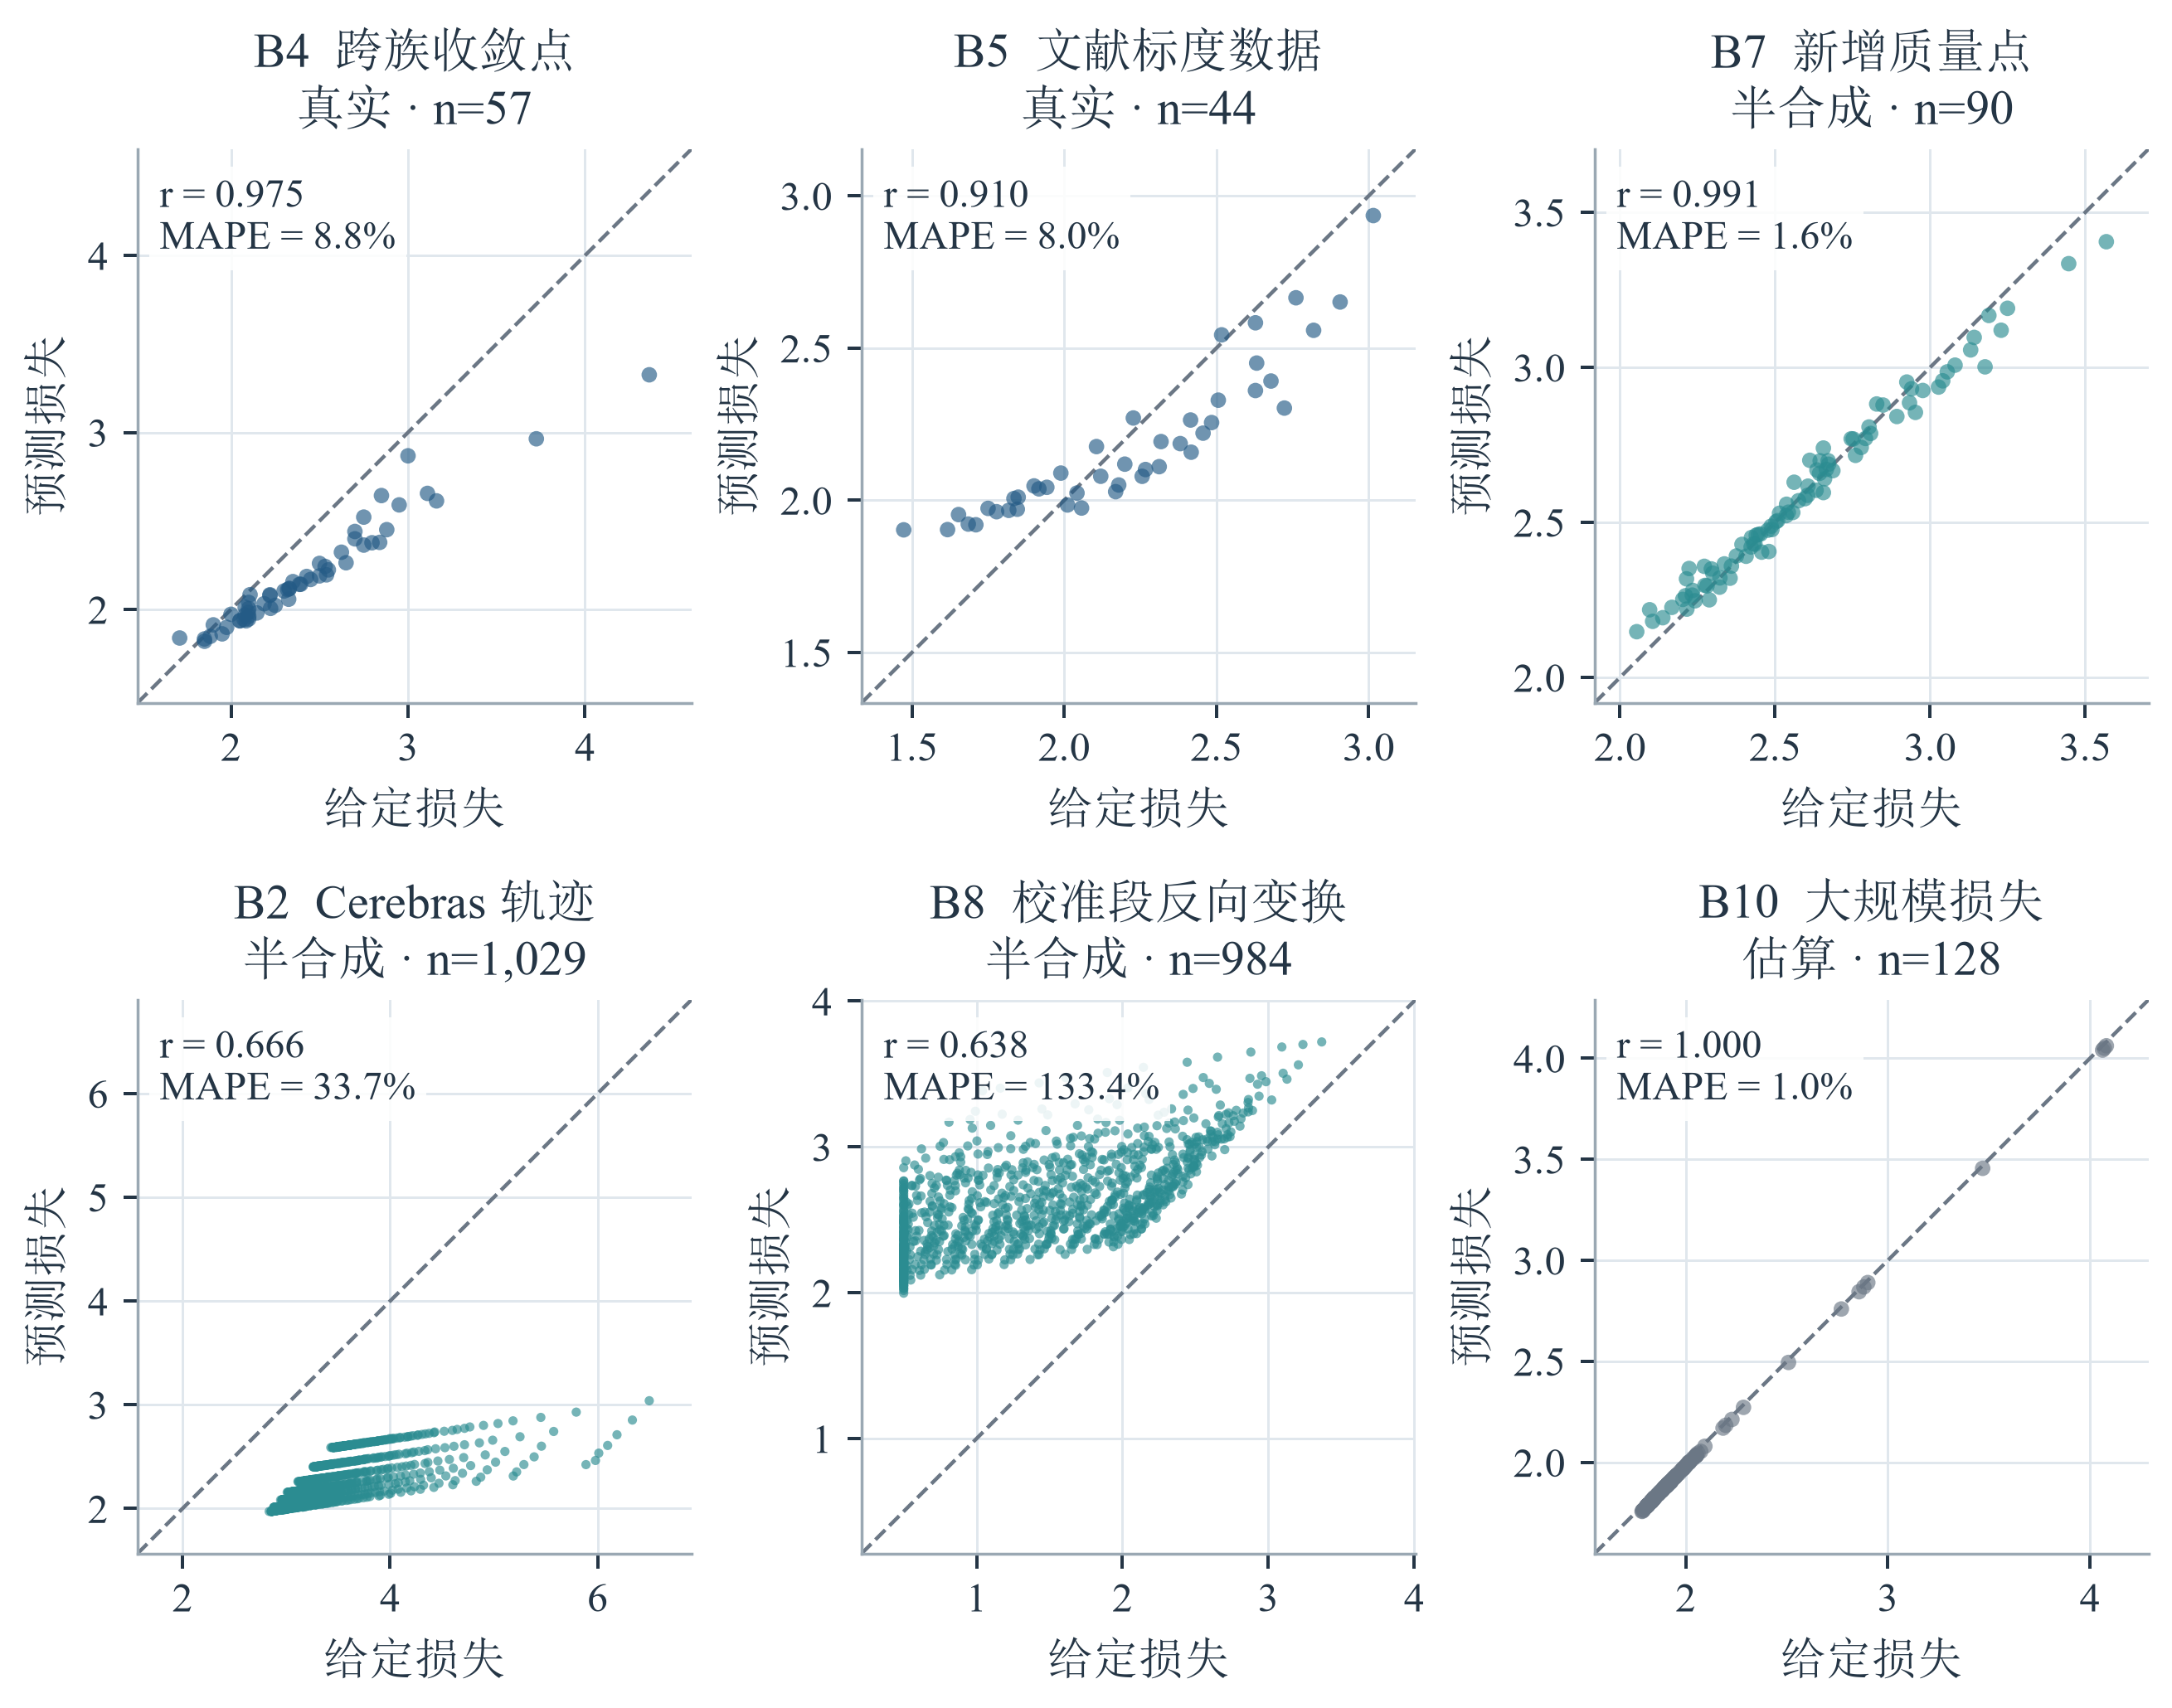
\includegraphics[width=0.98\textwidth]{../求解/问题二/图片/图2_广义标度律验证.png}
  \caption{不同数据来源的有符号相对误差分布}
  \label{fig:p2_general}
\end{figure}

\begin{samepage}
表\ref{tab:p2_val}中，B4 与 B5 的相关系数分别为 $0.975$、$0.910$，MAPE 分别为 $8.8\%$、$8.0\%$。两组结果表明，模型能够跟随部分跨族规模变化，但具体损失值仍有偏差，使用时不能只看相关性高低。
\par
\end{samepage}

\begin{samepage}
B7 的 90 个新增点得到 MAPE $1.6\%$，表明质量关系在同一半合成设定下可作一定扩展。B10 的损失来自估算，对照时统一取 $Q=1$，因而只检查估算关系是否接近，既不检验质量项，也不能作为独立实验。
\par
\end{samepage}

\begin{samepage}
B2 的 MAPE 为 $33.7\%$，B8 校准段在翻转评分后仍达 $133.4\%$。B8 还包含低于本模型渐近下限的损失。可见，改变质量方向并不足以统一这些来源，损失尺度或数据生成方式的差别仍会限制模型使用。
\par
\end{samepage}

\begin{samepage}
数值结论应结合估计所覆盖的范围使用。B1 的 $N$ 约为 $0.07$--$12$B，$D$ 为 $0.134$--$299.893$B tokens；B6 对应 $0.07$--$11.97$B 和 $10$--$600$B tokens。质量效应主要由 B6/B7 半合成实验支持，更大规模的估算记录只能检查外推关系的一致程度。
\par
\end{samepage}


\begin{samepage}
\textbf{4.大规模模型的对应与外推范围}\par\nopagebreak[4]
大规模对照先按 B9 模型名称与 B10 模型族名称匹配。B10 的 128 条记录均在 B9 找到唯一对应，且 $N$、$D$ 逐条相同。B9 原有 132 条，另外 4 条的数据量记为 0，也没有 B10 损失，所以不参加比较。匹配后的规模分组见表\ref{tab:p2_large}。
\par\nopagebreak[4]

\begin{table}[H]
  \centering
  \caption{大规模匹配样本的覆盖范围与估算偏差}
  \label{tab:p2_large}
  \renewcommand{\arraystretch}{1.15}
  \begin{tabularx}{0.94\textwidth}{@{}>{\raggedright\arraybackslash}X*{3}{>{\centering\arraybackslash}p{0.19\textwidth}}@{}}
    \toprule
    参数规模区间 $N$/B & $[100,300)$ & $[300,1000)$ & $[1000,10000]$ \\
    \midrule
    成功匹配记录数 & 65 & 43 & 20 \\
    最小数据量 / B tokens & 1.3 & 0.3 & 0.1 \\
    最大数据量 / B tokens & $36{,}000$ & $30{,}000$ & $36{,}000$ \\
    MAPE / \% & 0.94 & 1.08 & 1.12 \\
    \bottomrule
  \end{tabularx}
  \par\smallskip
  \begin{minipage}{0.94\textwidth}\normalsize
  注：B9 元数据与 B10 损失按名称匹配；统一取 $Q=1$，MAPE 比较本文预测与 B10 估算值。数据量上下限为各组记录的实际极值。
  \end{minipage}
\end{table}
\end{samepage}

匹配记录的规模为 $100$--$10{,}000$B，均超过主拟合范围。各组误差约为 $1\%$，说明两种估算关系接近。由于 B10 同样由标度律生成，低误差不能代替真实大模型训练验证，更不能证明质量效应在这一范围内仍然成立。


\textbf{5.质量投入的局部收益与规模替代}\par\nopagebreak[4]
下面选取两个参考配置，比较各项投入的小幅变化。表\ref{tab:p2_subst}同时列出弹性和质量--参数等效增量比，前者比较相同比例变化的影响，后者给出相同损失降幅下的局部换算。


\begin{table}[H]
  \centering
  \caption{两个参考情景下的局部敏感度与等效增量比}
  \label{tab:p2_subst}
  \renewcommand{\arraystretch}{1.18}
  \begin{tabularx}{0.94\textwidth}{@{}>{\raggedright\arraybackslash}X*{2}{>{\centering\arraybackslash}p{0.25\textwidth}}@{}}
    \toprule
    指标 & \makecell{参考情景一\\$N_0=1,\ D_0=100$\\$Q_0=0.6$} & \makecell{参考情景二\\$N_0=12,\ D_0=300$\\$Q_0=0.6$} \\
    \midrule
    参数量弹性 $\varepsilon_N$ & $-0.0491$ & $-0.0248$ \\
    数据量弹性 $\varepsilon_D$ & $-0.0383$ & $-0.0321$ \\
    质量弹性 $\varepsilon_Q$ & $-0.0838$ & $-0.0953$ \\
    局部等效增量比 $R_{NQ}$ & 2.844 & 76.838 \\
    \bottomrule
  \end{tabularx}
  \par\smallskip
  \begin{minipage}{0.94\textwidth}\normalsize
  注：$N_0$ 以 B 参数计，$D_0$ 以 B tokens 计；弹性无量纲，$R_{NQ}$ 的单位为 B/单位质量。弹性保留方向，图中展示其绝对值。
  \end{minipage}
\end{table}

\begin{samepage}
在 $(N_0,D_0,Q_0)=(1,100,0.6)$ 处，质量弹性的绝对值约为参数弹性的 $1.7$ 倍，即同样小比例的改善中，质量对应更大的损失降幅。两个参考配置的局部替代率分别为 $2.844$、$76.838$ B/单位质量。将质量增量 $0.1$ 代入一阶近似，得到等效扩参数量 $0.284$B、$7.684$B。这只是损失效果的近似比较；实际有限变化应按式\eqref{eq:p2_finite}计算，并检查是否超出拟合规模，不能将其直接当作等成本配置。
\par
\end{samepage}

图\ref{fig:p2_margin}把参考位置的变化展开。前两图分别展示参数、质量的边际导数绝对值，由于单位不同，两图数值不能直接比较。第三图使用无量纲弹性，能够比较两个参考点上相同比例投入带来的影响。

\begin{figure}[!htbp]
  \centering
  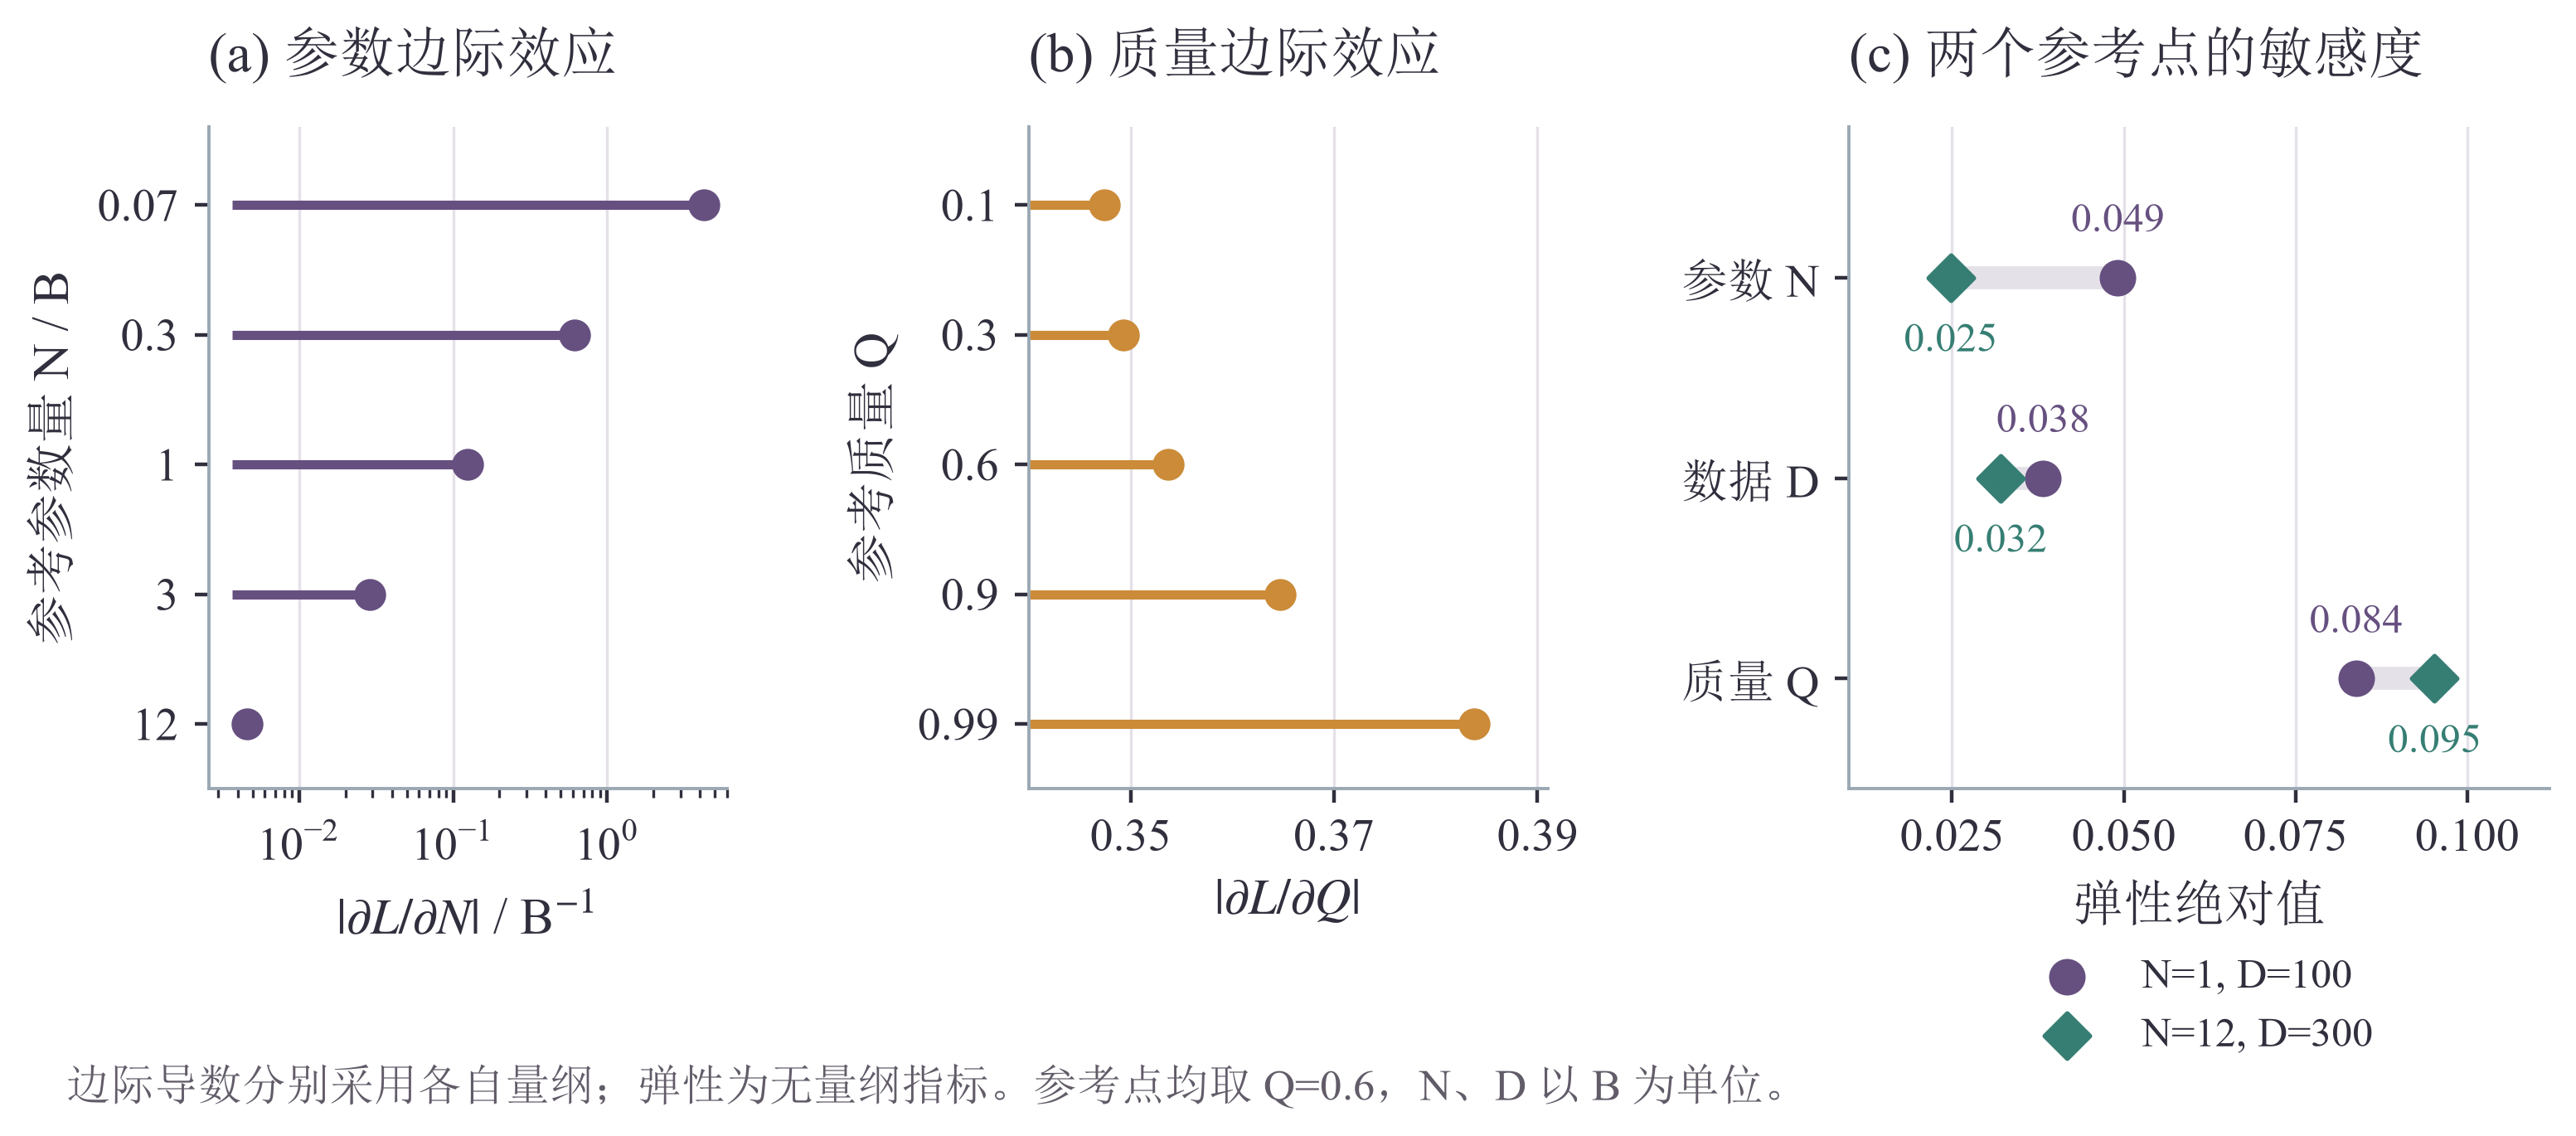
\includegraphics[width=0.98\textwidth]{../求解/问题二/图片/图4_边际效用对比.png}
  \caption{参考位置的边际效应与弹性对比}
  \label{fig:p2_margin}
\end{figure}

\begin{figure}[!htbp]
  \centering
  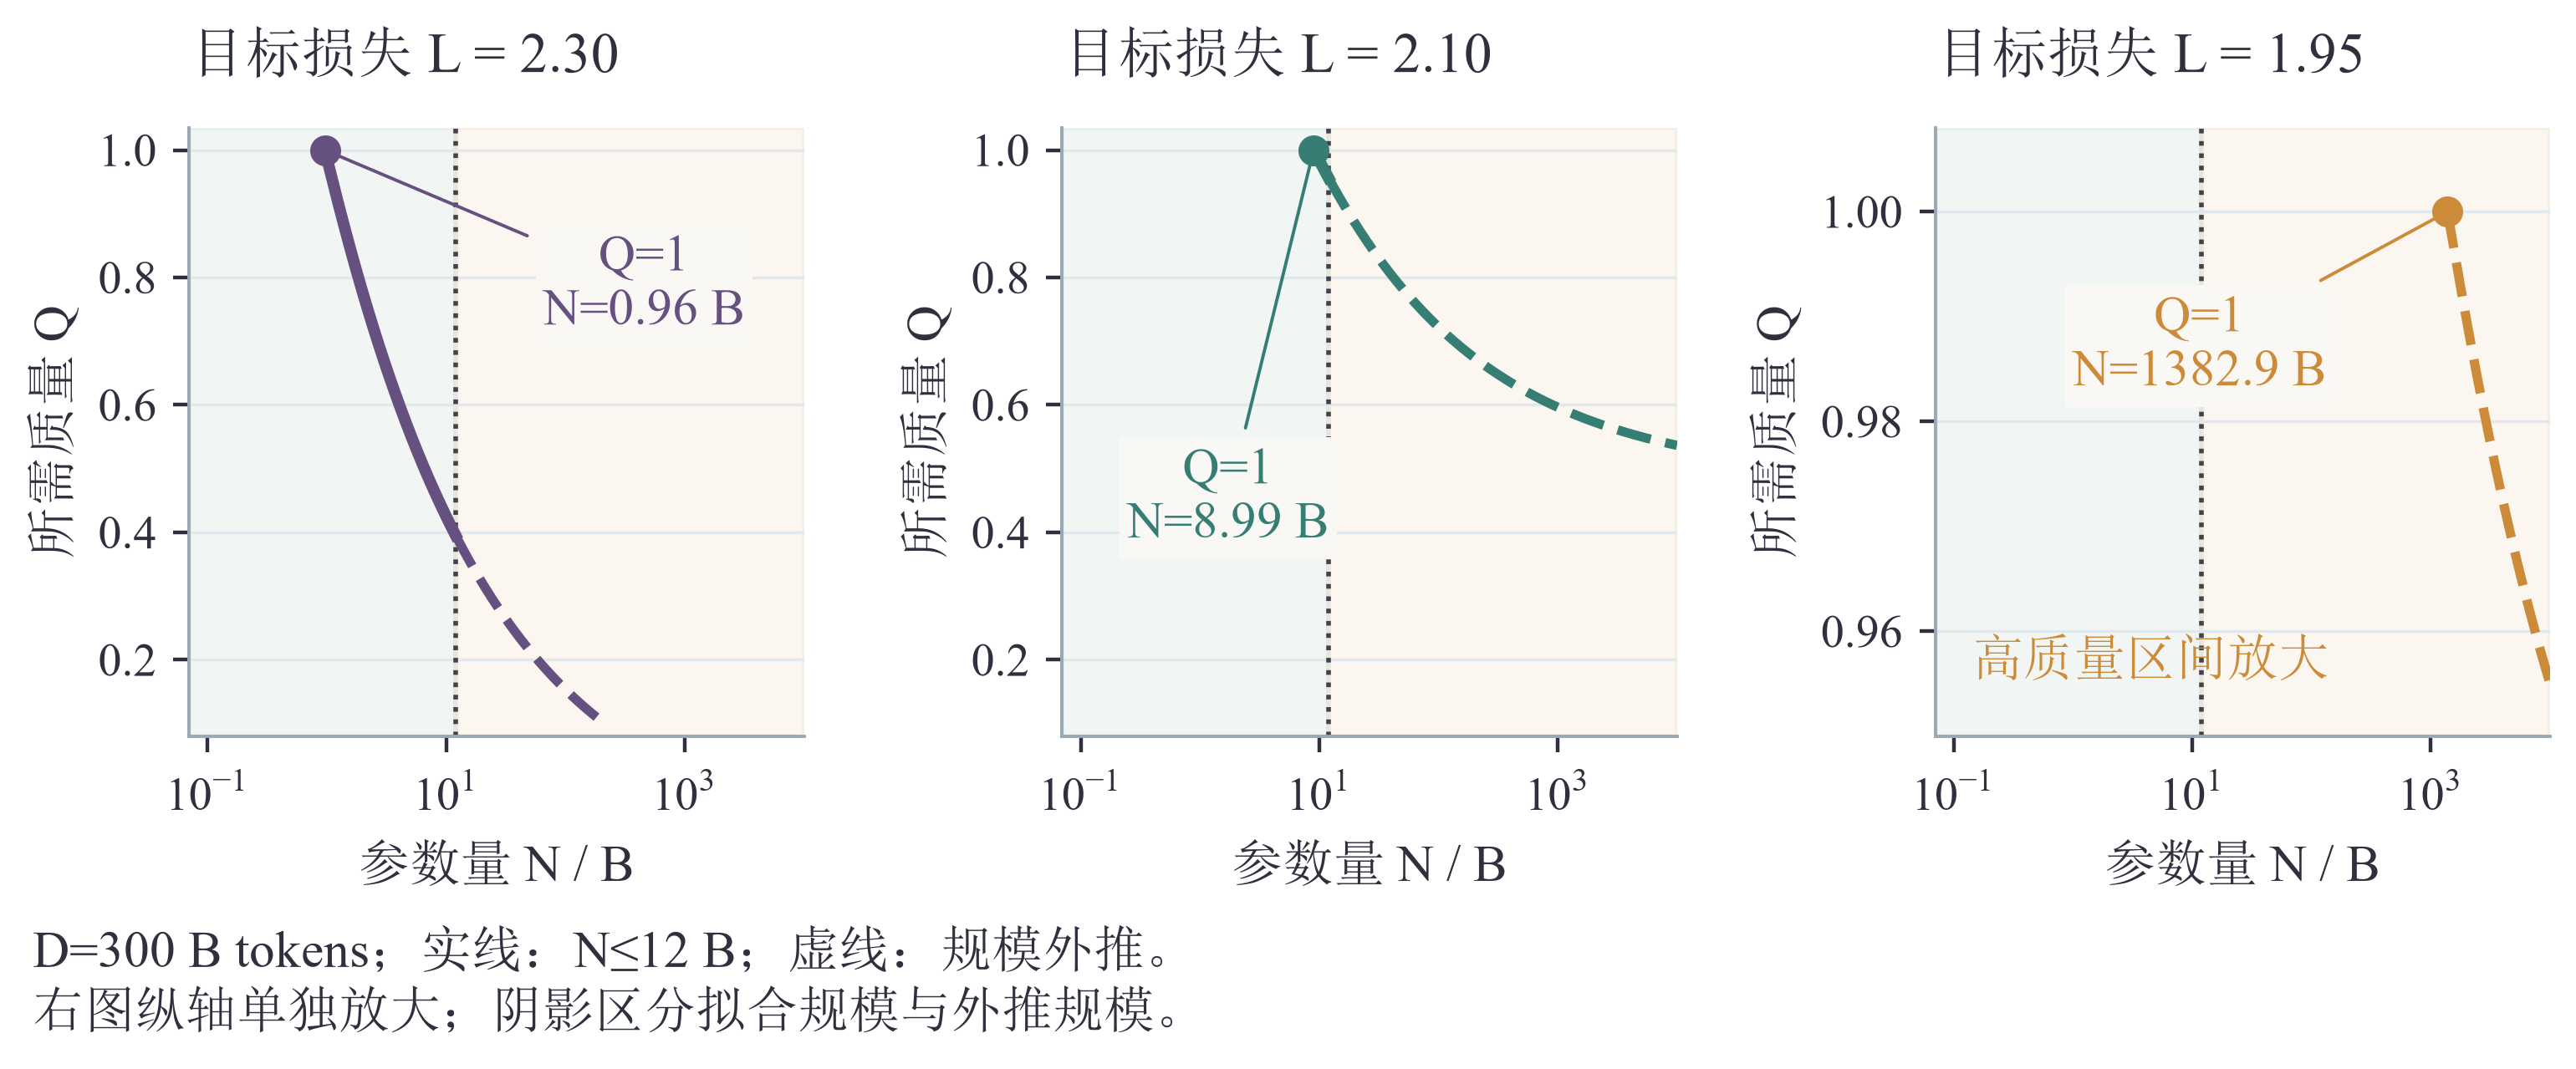
\includegraphics[width=0.98\textwidth]{../求解/问题二/图片/图5_质量参数替代.png}
  \caption{三个目标损失下的规模--质量配置边界}
  \label{fig:p2_subst}
\end{figure}

\begin{samepage}
固定 $D=300$B tokens 后，还可以反求达到目标损失需要的质量，见图\ref{fig:p2_subst}。三个子图各对应一个目标，横轴为参数量，纵轴为质量；实线在主拟合范围内，虚线为外推。对于 $L=1.95$，图中特别放大了高质量区间，并将参数轴延至 $10^4$B 以展示理论边界，这不表示该规模在工程上可行。
\par
\end{samepage}

\begin{samepage}
质量端点需另作处理。估计值 $\gamma=0.9779<1$ 使 $|\partial L/\partial Q|$ 在 $Q<1$ 时逐渐增大，并在 $Q\to1^-$ 时发散。因此，接近质量上界时不能直接用该导数作投入建议，边际效应的数值解释应限于远离端点的位置。
\par
\end{samepage}

\begin{samepage}
\textbf{6.领域效应与配比衔接}\par\nopagebreak[4]
为观察领域之间的关系，图\ref{fig:p2_dom}左侧按 $d_{ij}=\sqrt{2-2s_{ij}}$ 对 17 个训练领域作平均连接聚类；右侧列出相似度最高和最低的各四对领域，用绿色和金色分别表示作用趋同和相反。该图比较的是各域影响验证任务的方式，并不检验混合使用是否产生额外增益。
\par
\end{samepage}

\begin{figure}[!htbp]
  \centering
  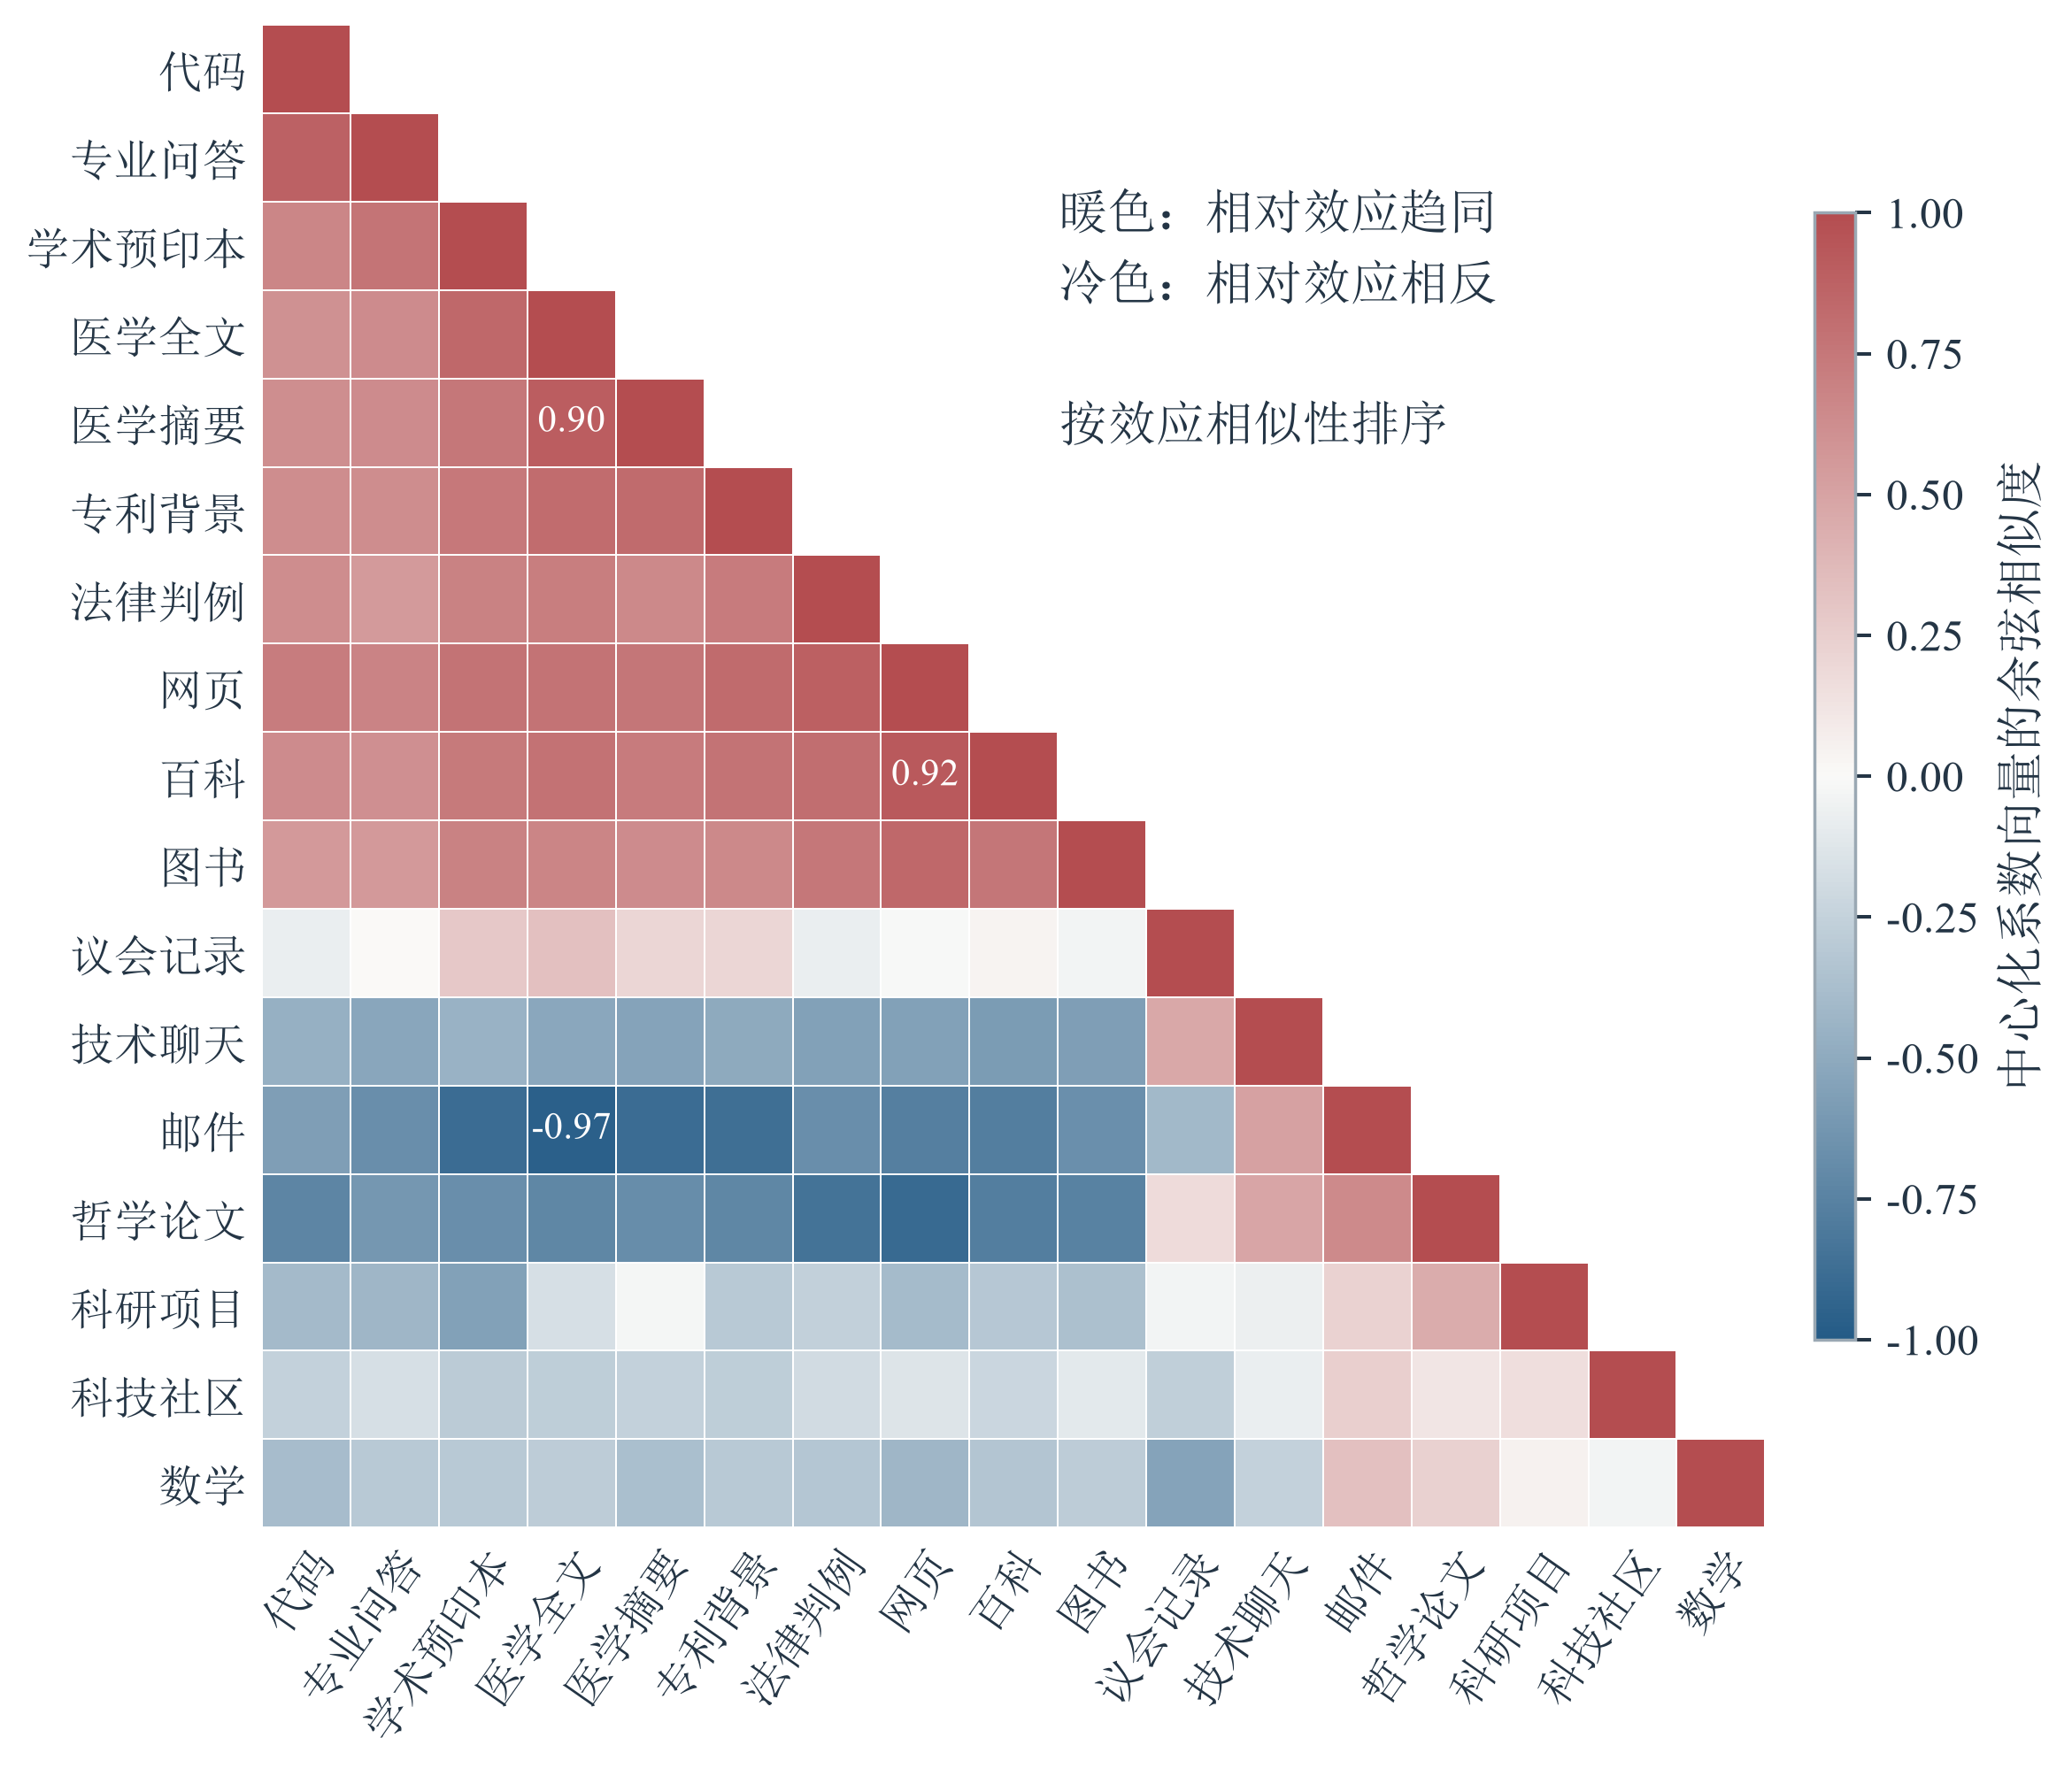
\includegraphics[width=0.98\textwidth]{../求解/问题二/图片/图6_领域替代互补.png}
  \caption{训练领域效应聚类与典型领域对比较}
  \label{fig:p2_dom}
\end{figure}

图\ref{fig:p2_dom}中，百科与网页的相似度为 $0.925$，医学全文与医学摘要为 $0.903$，说明它们在 13 个任务上的相对作用接近；医学全文与邮件为 $-0.967$，表明两者偏向不同任务。若要决定能否替换，还需保留作用大小与任务权重。设从领域 $i$ 向 $j$ 转移占比 $h$，保持总占比不变并满足 $0\leq h\leq p_i$，则预测加权损失变化为
\begin{equation}
  \Delta\widehat L_A=h\,\bm w^{\mathsf T}(\bm a_j-\bm a_i),
\end{equation}
这里 $\bm w$ 是验证领域权重。上式为负时，替换有利于总体表现；为零时效果相当，为正时表现下降。因而，相似度接近并不保证等量替换无损，相反的作用方向也只表示任务之间存在取舍。原模型没有交互项，不能再从中推断两域混合后的额外互补收益。


对问题一推荐配比与参考配比作同口径比较，线性模型给出的加权损失差为
\[
  M=\hat L(\bm p_{\mathrm{rec}})-\hat L(\bm p_{\mathrm{ref}})=-0.1988.
\]
\begin{samepage}
$M$ 来自附件 A 的任务集合和权重。只有在配比效果能够与规模、质量分开，且损失差可在来源之间迁移时，才能将 $M(\bm p)$ 加入广义标度律。前面的检验已显示不同来源存在偏差，所以 $0.1988$ 是当前条件下的损失差，不能保证各个规模都获得同样改善。
\par
\end{samepage}

\begin{samepage}
在上述分离与迁移条件下，规模、质量和配比的关系可合写为
\par\nopagebreak[4]
\begin{equation}
  \begin{aligned}
    L(N,D,Q,\bm p)&=E+AN^{-\alpha}+BD^{-\beta}+C(1-Q)^\gamma+M(\bm p),\\
    M(\bm p)&=\sum_{i=1}^{17}(p_i-p_{\mathrm{ref},i})\,\bm w^{\mathsf T}\bm a_i.
  \end{aligned}
\end{equation}
\end{samepage}
参考配比满足 $M(\bm p_{\mathrm{ref}})=0$。固定配比后，$M$ 只改变损失的整体水平，$N,D,Q$ 的边际导数与等损失替代条件保持不变；本节弹性均在参考配比下计算。若后续直接代入问题一评分，还要假设它与附件 B 的质量尺度能够衔接，这一假设并不能由加性公式自动保证。


本问为预算分配提供了损失函数，也说明了如何使用：模型越大，继续扩参数的边际收益越小；改善质量可以替代多少参数，则取决于初始配置。跨族与文献数据仍有 $8.8\%$、$8.0\%$ 的 MAPE，因此后续配置除了使用拟合值，还需保留对评分尺度、数据来源和外推范围的限制。
\endgroup
